%% main.tex — Compact Bonnet Pairs: Computational Extension to 998 Seeds
%% and an Asymptotic Law for the Closure Parameter
%%
%% Target: Experimental Mathematics (Taylor & Francis)
%% arXiv: math.DG / math.NA
%%
\documentclass[11pt,a4paper]{article}

%% ── Packages ─────────────────────────────────────────────────────────
\usepackage[utf8]{inputenc}
\usepackage[T1]{fontenc}
\usepackage{amsmath,amssymb,amsthm,mathtools}
\usepackage{thmtools}
\usepackage{enumitem}
\usepackage{booktabs}
\usepackage{array}
\usepackage{graphicx}
\usepackage[svgnames]{xcolor}
\usepackage[colorlinks,citecolor=DarkBlue,linkcolor=DarkRed,urlcolor=DarkBlue]{hyperref}
\usepackage{cleveref}
\usepackage[protrusion=true,expansion=false]{microtype}
\usepackage{geometry}
\geometry{margin=2.5cm}

%% ── Theorem environments (BHS style) ──────────────────────────────
\theoremstyle{plain}
\newtheorem{theorem}{Theorem}[section]
\newtheorem{proposition}[theorem]{Proposition}
\newtheorem{lemma}[theorem]{Lemma}
\newtheorem{corollary}[theorem]{Corollary}
\newtheorem{conjecture}[theorem]{Conjecture}

\theoremstyle{definition}
\newtheorem{definition}[theorem]{Definition}
\newtheorem{observation}[theorem]{Observation}

\theoremstyle{remark}
\newtheorem{remark}[theorem]{Remark}

%% ── Notation ────────────────────────────────────────────────────────
\DeclareMathOperator{\Real}{Re}
\DeclareMathOperator{\Imag}{Im}
\DeclareMathOperator{\tr}{tr}
\newcommand{\vt}[1]{\vartheta_{#1}}     % theta functions
\newcommand{\CC}{\mathbb{C}}
\newcommand{\RR}{\mathbb{R}}
\newcommand{\ZZ}{\mathbb{Z}}
\newcommand{\NN}{\mathbb{N}}
\newcommand{\HH}{\mathbb{H}}            % quaternions
\newcommand{\T}{\mathbb{T}}             % torus
\newcommand{\Sp}{\mathbb{S}}            % sphere
\newcommand{\dd}{\mathrm{d}}
\newcommand{\ee}{\mathrm{e}}
\newcommand{\ii}{\mathrm{i}}
\newcommand{\abs}[1]{\lvert #1 \rvert}
\newcommand{\norm}[1]{\lVert #1 \rVert}
\newcommand{\Oo}{\mathcal{O}}

%% ── Title ───────────────────────────────────────────────────────────
\title{%
  Compact Bonnet Pairs for $k$-fold Tori:\\
  998 Computed Seeds and a Validated $k^{-1/2}$
  Asymptotic Law}

\author{%
  Oleksiy Babanskyy
}
\date{}

%% ═════════════════════════════════════════════════════════════════════
\begin{document}
\maketitle

%% ── Abstract ────────────────────────────────────────────────────────
\begin{abstract}
Bobenko, Hoffmann, and Sageman-Furnas~\cite{BHS25,BHS-comp} constructed
compact Bonnet pairs from isothermic tori whose closing conditions
reduce to a system on a genus-one spectral curve.
Working on a single reference branch (gauge $s_1 = -8.5$),
we solve these conditions for all fold numbers
$k = 3,\ldots,1000$, producing $998$ seeds verified
by a four-gate numerical protocol
(with retraction-form validation on representative seeds).
A step-$10$ continuation extends the dataset
to $k > 6\times 10^5$, with typical agreement
$\lvert\delta_k\sqrt{k} - A\rvert \approx 1.4$~ppm (parts per million)
(up to~$\approx 37$~ppm at isolated wobble points).
The principal finding is the asymptotic law
\[
  \delta_k = \frac{A}{\sqrt{k}}\,\Bigl(1 - \frac{c_1}{k}
  + \Oo(k^{-2})\Bigr),
  \qquad A = 7.081\,416\,491\,399\,252\,576 \pm 3 \times 10^{-18},
\]
supported by Richardson extrapolation and a formal-analytic derivation
with numerically verified remainder for $k \ge 100$.
The cross-ratio at~$\omega_{\mathrm{crit}}$ satisfies
$\lvert\arg(\mathrm{CR})\rvert \cdot k \to 4$ (\cref{rem:CR-sign}),
and the modular parameter of the spectral curve is conjectured to satisfy
\[
  \tau_{\mathrm{spec}}(k)
  \;=\; -\tfrac{1}{2} + \ii\,\frac{\ln(4k)}{\pi},
\]
verified to $6$~significant digits for $k \le 200$
(\cref{conj:tau-spec}), suggesting a closed-form relation between
the fold number~$k$ and the conformal type of the spectral curve.
PSLQ at $19$~digits fails to identify $A$ or the limiting~$C_2$.
\end{abstract}

\smallskip
\noindent\textbf{Keywords:}
  Bonnet pairs, isothermic tori, theta functions, spectral curve,
  closing conditions, asymptotic analysis, retraction form.

\smallskip
\noindent\textbf{MSC\,2020:}
  53A05, 53C42, 33E05, 65D30, 34M55.

%% ═════════════════════════════════════════════════════════════════════
\section{Introduction}\label{sec:intro}
%% ═════════════════════════════════════════════════════════════════════

\subsection{The Bonnet problem}
A classical problem due to Bonnet~\cite{Bon67} asks whether two
non-congruent immersions $f^+, f^- \colon \Sigma \to \RR^3$ of a
surface~$\Sigma$ can share the same induced metric and mean curvature
function.  When such a pair exists, $f^+$ and~$f^-$ are called a
\emph{Bonnet pair}.  Lawson and Tribuzy~\cite{LT81} showed that
if~$\Sigma$ is compact, a Bonnet pair must be a two-parameter family
(which cannot occur for genus $\geq 1$) or an isolated pair.

The problem remained open for compact surfaces for over a century.
Kamberov, Pedit, and Pinkall~\cite{KPP98} established a decisive link:
a surface admitting a Bonnet mate must be isothermic.  In the landmark
work~\cite{BHS25}, Bobenko, Hoffmann, and Sageman-Furnas (hereafter
BHS) resolved the problem by constructing compact Bonnet pairs
from isothermic tori with one family of planar and one family of
spherical curvature lines.  Their companion paper~\cite{BHS-comp}
provides the complete classification of such isothermic tori.

\subsection{The closing conditions}
The construction in~\cite{BHS25} reduces the existence of compact
Bonnet pairs to a system of transcendental equations on an elliptic
spectral curve.  Let $\tau = \tfrac{1}{2} + \ii\lambda$,
$\lambda \in (0,\lambda_0)$ with $\lambda_0 \approx 0.3547$, be the
lattice parameter of rhombic type, and let $\omega \in (0,\pi/4)$ be
the unique critical point of $\vt{2}(\cdot|\tau)$ in this interval.

For each fold number $k \geq 3$, one seeks parameters $(\delta, s_2)$
with $s_1$ fixed (a gauge choice), such that:
\begin{enumerate}[label=(\roman*),nosep]
\item the \emph{theta-half periodicity} condition holds
  (ensuring that the frame $\Phi(v)$ rotates by exactly $2\pi/k$ per
  fundamental piece), and
\item the \emph{axial period integral} vanishes
  (ensuring that the surface closes without translational drift
  along the rotation axis).
\end{enumerate}
These conditions are Equations~(82)--(83) of~\cite{BHS-comp}; we
recall their precise form in~\cref{sec:periodicity}.

\subsection{Contributions}
Our contributions are as follows.
\begin{enumerate}[label=\textbf{C\arabic*}.,nosep]
\item \textbf{Computational extension.} We solve conditions~(i)--(ii)
  for all $k = 3,\ldots,1000$, producing $998$ Bonnet-pair seeds
  $(\delta_k, s_{2,k})$ at gauge $s_1 = -8.5$.  Every solution is
  verified to residual $< 10^{-10}$.  A step-$10$ sampled
  continuation supports the asymptotic law to $k > 6\times 10^5$.
\item \textbf{Asymptotic law.}
  The closure parameter satisfies
  $\delta_k = (A/\sqrt{k})(1 - c_1/k + \Oo(k^{-2}))$
  with $A = 7.081\,416\,491\,399\ldots$ ($19$~significant digits;
  see~\eqref{eq:A}).
  Richardson extrapolation reveals a further correction
  $c_3/k^2$ with $c_3 \approx 0.75$ (\cref{obs:c3}).
  Running-exponent and Richardson analyses are given in full.
  A formal spectral-curve derivation yields the closed-form
  amplitude $A^2 = 2\tilde Q_2^2\,\Delta s^2/(Z_0\,\tilde Q_2'\,Q_3)$,
  agreeing with Richardson extrapolation to $6$~ppm
  (\cref{sec:spectral-remainder}).
\item \textbf{Retraction form validation.}
  We implement the retraction form of~\cite{BCHR25} with analytic
  derivatives and confirm it on $8$ representative seeds;
  the stereographic identity $\abs{x}=1$ holds to machine
  epsilon, while the differential gates (closure, cross condition)
  are satisfied to five to six significant digits.
\item \textbf{Analytical identities.}
  We verify $\abs{x} = 1$ on the stereographic lift (a tautology
  of the construction, used as a pipeline sanity check),
  verify conformality $\abs{x_u}^2 = \abs{x_v}^2$ to
  $8.5 \times 10^{-7}$, and observe the off-diagonal
  II-discrepancy $b = 1 + \Oo(\Delta u^2)$ for the
  second fundamental form.
\item \textbf{Moduli-space flow.}
  Implicit differentiation of the periodicity system yields the
  flow ODE $d(\delta, s_2)/ds_1 = -J^{-1}\,\partial F/\partial s_1$,
  which reproduces $121$ sweep points to $< 0.002\%$.
  The Jacobian is a saddle ($\lambda_+ > 0$, $\lambda_- < 0$)
  at all tested sweep points, with anisotropy ratio $\lambda_+/\abs{\lambda_-}
  \sim k^{1.49}$; the flow terminates at a fold singularity
  $s_1^*$ (\cref{sec:flow}).
\item \textbf{Spectral invariants.}
  The quartic $Q(s)$ preserves the root type
  ($2$ real $+ 2$ complex conjugate) along the entire flow.
  At the critical point $\omega_{\mathrm{crit}}$ of
  $\vt{2}(\cdot|\tau)$, the full complex cross-ratio of the
  four roots is numerically constant (to $< 10^{-11}$), with $\lvert\arg(\mathrm{CR})
  \rvert \cdot k \to 4$~rad as $k \to \infty$
  (\cref{rem:CR-sign} discusses the sign convention).
  This constancy is a sharp property of $\omega_{\mathrm{crit}}$
  (not a consequence of $\tau$ being fixed), demonstrated by a
  systematic $\omega$-scan (\cref{sec:spectral-inv}).
\item \textbf{Negative results.}
  PSLQ fails to identify $A$ against $37$ basis sets
  (up to $11$ elements each) including
  powers of~$\pi$, the lattice parameter~$\omega$, theta-null
  values, Catalan's constant, elliptic integrals, Eisenstein
  series, the $j$-invariant, and Dedekind's~$\eta$.
  For $C_2 = s_{2,\infty}$, an arbitrary-precision solver
  ($40$-digit \texttt{mpmath} arithmetic, Gauss--Legendre
  quadrature, $116$ sparse $k$-values up to~$5000$)
  yields $C_2$ to $19$~digits; PSLQ with
  $\mathrm{maxcoeff} = 10\,000$ returns ``no relation'' on
  all $36$~basis sets, including elliptic integrals, Eisenstein
  series, the $j$-invariant, and Dedekind's~$\eta$
  (\cref{prop:pslq-C2-neg}).
  No conserved quantity among natural moduli-space functions
  ($\delta^2 Q_3$, $\Delta(Q)$, \ldots) is found along the flow:
  the gauge flow is not Hamiltonian in these coordinates.
\item \textbf{Spectral modular parameter.}
  The modular parameter of the spectral curve
  $w^2 = Q(s)$ at~$\omega_{\mathrm{crit}}$ is conjectured to satisfy
  $\tau_{\mathrm{spec}}(k) = -\tfrac12 + \ii\,\ln(4k)/\pi$,
  verified to $6$~digits for $k \le 200$, with
  nome $q_{\mathrm{spec}} = -\ii/(4k)$ and
  $\lambda(\tau_{\mathrm{spec}}) = \mathrm{CR}_k$
  to~$10^{-11}$ (\cref{conj:tau-spec}).
  The connection constant $C_0$ in Jimbo's logarithmic
  asymptotics is conjectured but remains numerically
  inaccessible (\cref{conj:C0}).
\end{enumerate}

\subsection{Relationship to prior and concurrent work}
Dornic and Conte~\cite{DC26} establish that Painlev\'e~VI
with Manin coefficients $[0,0,0,0]$ governs \emph{generic}
(non-compact) Bonnet surfaces: the mean curvature is a PVI
tau-function and the equation arises from the Bobenko--Eitner
Lax pair via a double Kitaev folding.
The variable~$\ell$ in~\cite{DC26} is the Ising scaling time,
\emph{not} the fold number~$k$; the bridge between PVI and
the $k$-fold periodicity condition remains open
(see~\cref{sec:open}, OP3).

The retraction form originates in the work of Burstall, Hoffmann,
Pedit, and Sageman-Furnas~\cite{BCHR25} on isothermic
surfaces in $S^4$, projected to $\RR^3$ via stereographic projection.

\subsection{Outline}
\Cref{sec:prelim} recalls theta functions and the spectral-curve
formalism of~\cite{BHS-comp}.  \Cref{sec:periodicity} states the
periodicity conditions precisely.  \Cref{sec:computational} describes
the computational pipeline.  \Cref{sec:extension} presents the
$998$-seed dataset and reproduction of known examples.
\Cref{sec:asymptotic} contains the asymptotic analysis.
\Cref{sec:analytical} establishes the geometric identities.
\Cref{sec:flow} derives the moduli-space flow ODE and analyses
the spectral invariants along the flow.
\Cref{sec:retraction} validates the retraction form.
\Cref{sec:open} discusses open problems.

These components form a unified computational study: the dataset
(\cref{sec:extension}), asymptotic law (\cref{sec:asymptotic}), and
spectral invariants (\cref{sec:flow}) are interdependent, with the
geometric identities (\cref{sec:analytical}) and retraction-form
validation (\cref{sec:retraction}) providing independent
cross-checks.

%% ═════════════════════════════════════════════════════════════════════
\section{Mathematical Preliminaries}\label{sec:prelim}
%% ═════════════════════════════════════════════════════════════════════

We work on an elliptic curve with rhombic lattice
$\Lambda = \pi\ZZ + \pi\tau\ZZ$, where
$\tau = \tfrac12 + \ii\lambda$, $\lambda \in (0,\lambda_0)$ and
$\lambda_0 \approx 0.3547$ is the unique value with
$\vt{2}''(0|\tau_0) = 0$~\cite[Lemma~8]{BHS-comp}.
Our reference lattice parameter is $\lambda = 25/78 \approx 0.3205$
(i.e.\ $\tau = \tfrac{1}{2} + \tfrac{25}{78}\,\ii$).

\subsection{Theta functions}\label{sec:theta}
We use the four Jacobi theta functions in the
Whittaker--Watson~\cite{WW27} convention:
\begin{align}
  \vt{1}(z,q) &= 2\sum_{n=0}^{\infty} (-1)^n\, q^{(n+1/2)^2}
    \sin\bigl((2n+1)z\bigr), \label{eq:theta1} \\
  \vt{2}(z,q) &= 2\sum_{n=0}^{\infty} q^{(n+1/2)^2}
    \cos\bigl((2n+1)z\bigr), \label{eq:theta2} \\
  \vt{3}(z,q) &= 1 + 2\sum_{n=1}^{\infty} q^{n^2}
    \cos(2nz), \label{eq:theta3} \\
  \vt{4}(z,q) &= 1 + 2\sum_{n=1}^{\infty} (-1)^n\, q^{n^2}
    \cos(2nz), \label{eq:theta4}
\end{align}
with nome $q = \ee^{\ii\pi\tau}$.  For the rhombic lattice,
$q = \ii\,\ee^{-\pi\lambda}$.

\begin{remark}
  All theta series are computed to $50$ terms following
  standard algorithms~\cite{Dee11}; for
  $\lambda \geq 0.3$ this gives $\abs{q}^{2500} < 10^{-16}$, ensuring
  machine-precision convergence.
\end{remark}

\subsection{Spectral curve coefficients}\label{sec:coeff}
Following~\cite[Section~3.2]{BHS-comp}, the Lam\'e--Riccati
coefficients are:
\begin{align}
  R(\omega) &= \frac{2\,\vt{2}(\omega)^2}
    {\vt{1}'(0)\,\vt{1}(2\omega)},
  \label{eq:Romega} \\
  U(\omega) &= -\frac{\vt{1}'(0)\,\vt{1}(2\omega)}
    {2\,\vt{2}(\omega)^2}
  = -\frac{1}{R(\omega)},
  \label{eq:U} \\
  U'(\omega) &= -\frac{\vt{1}'(0)\,\vt{1}'(2\omega)}
    {2\,\vt{2}(\omega)^2},
  \label{eq:Uprime} \\
  U_1'(\omega) &= \frac{\vt{1}'(0)^2}
    {2\,\vt{2}(\omega)^2},
  \label{eq:U1prime} \\
  U_2(\omega) &= \frac{\vt{1}'(0)^2}{\vt{2}(\omega)^2}
    \biggl[
      \frac{\vt{1}(\omega)^2}{\vt{2}(0)^2}
    + \frac{\vt{4}(\omega)^2}{\vt{3}(0)^2}
    + \frac{\vt{3}(\omega)^2}{\vt{4}(0)^2}
    \biggr].
  \label{eq:U2}
\end{align}
These are the coefficients of the integer Lam\'e equation
$y'' = (C_1 - 8\theta)\,y$ from~\cite[Lemma~1]{BHS-comp}.

\subsection{The quartic spectral polynomial}\label{sec:Q}
Let $s = \ee^{-h(\omega,w)}$ denote the conformal factor evaluated at
the critical point $u=\omega$.  The two elliptic curves governing the
surface are:

\begin{definition}[Cubic spectral polynomial {\cite[Eq.~58]{BHS-comp}}]
\label{def:Q3}
\begin{equation}
  Q_3(s) \;=\; 2\,U_1'\,s^3 \;-\; U_2\,s^2
    \;-\; 2\,U'\,s \;-\; U^2.
  \label{eq:Q3}
\end{equation}
\end{definition}

\begin{definition}[Quartic spectral polynomial
  {\cite[Theorem~9]{BHS-comp}}]
\label{def:Q}
For parameters $\delta \in \RR \setminus \{0\}$ and
$s_1, s_2 \in \CC$ (either both real or complex conjugate), define
\begin{equation}
  Q(s) \;=\; -(s - s_1)^2(s - s_2)^2 \;+\; \delta^2\,Q_3(s).
  \label{eq:Q}
\end{equation}
This is a degree-$4$ polynomial in~$s$ with real coefficients.  Its
discriminant locus determines the genus of the spectral curve:
generically, $Q$ has four distinct roots and the spectral curve
$\mu^2 = Q(s)$ is elliptic (genus~$1$).
\end{definition}

\begin{remark}
  The polynomial $Q(s)$ governs the reparametrization function
  $w(v)$ through $v'(s) = \delta/\sqrt{Q(s)}$, while
  $w'(s) = 1/\sqrt{Q_3(s)}$~\cite[Corollary~6]{BHS-comp}.
  Together, they determine an isothermic torus with one family of
  planar and one family of spherical curvature lines.
\end{remark}


%% ═════════════════════════════════════════════════════════════════════
\section{Periodicity Conditions}\label{sec:periodicity}
%% ═════════════════════════════════════════════════════════════════════

For the isothermic cylinder to close into a $k$-fold torus, two
conditions must be satisfied simultaneously.  We follow the notation
of~\cite[Section~5.3]{BHS-comp}.
(Lemma~8 of~\cite{BHS-comp} establishes that the closing conditions
reduce to two real equations on $(\delta, s_2)$;
Lemma~9 verifies local uniqueness via the non-vanishing
Jacobian of the period map.)

\subsection{Theta-half periodicity}\label{sec:theta-half}

\begin{proposition}[Theta-half condition,
  {\cite[Eq.~82]{BHS-comp}}]
\label{prop:theta-half}
Let $s = \ee^{-h(\omega,w)}$ and let $\mathcal{V}$ denote the range
of~$s$ over one period of~$w(v)$.  The fundamental piece closes with
rotation angle $\theta = 2\pi/k$ if and only if
\begin{equation}
  F_{\mathrm{rat}}(\delta,s_2)
  \;\coloneqq\;
  \int_{\mathcal{V}} \frac{\delta}{\sqrt{Q(s)}} \;\dd s
  \;-\; \frac{2\pi}{k}
  \;=\; 0.
  \label{eq:F-rat}
\end{equation}
\end{proposition}

\subsection{Axial period integral}\label{sec:axial}

\begin{proposition}[Axial condition,
  {\cite[Eq.~83]{BHS-comp}}]
\label{prop:axial}
The translational drift along the rotation axis vanishes if and only if
\begin{equation}
  F_{\mathrm{ax}}(\delta,s_2)
  \;\coloneqq\;
  \int_{\mathcal{V}}
    \frac{Q_2(s)}{\sqrt{Q(s)}} \;\dd s
  \;=\; 0,
  \label{eq:F-ax}
\end{equation}
where $Q_2(s)$ is the axial numerator
(\cite[Eq.~86]{BHS-comp}):
\begin{equation}
  Q_2(s) \;=\; -(s - s_1)(s - s_2)
    \;+\; \delta^2\,U_1'(\omega)\,s.
  \label{eq:Q2}
\end{equation}
\end{proposition}

\begin{remark}
  Together, \cref{eq:F-rat,eq:F-ax} form a $2 \times 2$ nonlinear
  system in $(\delta, s_2)$ at each fixed $k$ and gauge~$s_1$.  We
  solve this system by a damped Newton method with numerical
  Jacobian~(\cref{sec:newton}).
\end{remark}


%% ═════════════════════════════════════════════════════════════════════
\section{Computational Framework}\label{sec:computational}
%% ═════════════════════════════════════════════════════════════════════

\subsection{Architecture overview}\label{sec:arch}
The computational pipeline consists of five independent modules:
\begin{enumerate}[nosep]
\item \texttt{theta\_functions}: evaluation of
  $\vt{1}$--$\vt{4}$ and their derivatives to $50$ terms,
  plus all spectral coefficients
  $R, U, U', U_1', U_2, Q_3, Q$~(\cref{sec:coeff,sec:Q}).
\item \texttt{theorem7\_periodicity}: the Newton solver for
  the system $F_{\mathrm{rat}} = F_{\mathrm{ax}} = 0$,
  with continuation in~$k$ and adaptive damping.
\item \texttt{analytic\_derivatives}: chain-rule derivatives
  of $\psi = \vt{1}'/\vt{1}$, the surface coordinates
  $f_u, f_v$, and the mean curvature~$H$.
\item \texttt{frame\_integrator}: eighth-order Dormand--Prince
  (DOP853) integration of the frame ODE
  $\Phi'(v) = \sqrt{1 - w'(v)^2}\,W_1(w(v))\,\mathbf{k}\,\Phi(v)$
  over one fundamental period.
\item \texttt{retraction\_form}: the Burstall et al.~\cite{BCHR25}
  construction $dF^+ = \tfrac12 \bar{x}\,\omega$,
  $dF^- = -\tfrac12 \bar{\omega}\,x$ with five quality gates.
\end{enumerate}
The elliptic and theta-function core (\texttt{theta\_functions})
was cross-validated against exact closed-form solutions of the
KdV and sine-Gordon equations, achieving residuals at the level
of machine precision ($< 10^{-15}$).

\subsection{Newton solver}\label{sec:newton}
The system~\eqref{eq:F-rat}--\eqref{eq:F-ax} is solved by a
$2 \times 2$ Newton iteration with the following features:
\begin{itemize}[nosep]
\item \textbf{Numerical Jacobian.}
  The $2 \times 2$ Jacobian matrix
  $J_{ij} = \partial F_i/\partial x_j$
  ($x = (\delta, s_2)$, $F = (F_{\mathrm{rat}}, F_{\mathrm{ax}})$)
  is computed by central finite differences with step sizes
  $h_{\delta} = \max(10^{-6},\, 10^{-6}\abs{\delta})$
  and $h_{s_2} = \max(10^{-6},\, 10^{-6}\abs{s_2})$.
  The solver uses \texttt{scipy.optimize.root} with
  \texttt{method='hybr'}.
\item \textbf{Elliptic integrals.}
  The integrals~\eqref{eq:F-rat}--\eqref{eq:F-ax} are evaluated
  over the real oval of $Q(s)$, i.e.\ the interval
  $[s^-,\, s^+]$ between the two real roots of~$Q$ that satisfy
  $Q(s) > 0$ in the interior and $s_1 \in [s^-,\, s^+]$.
  Endpoint singularities ($Q \to 0$ as square roots) are removed
  by the substitution $s = \tfrac12(s^- + s^+)
  + \tfrac12(s^+ - s^-)\sin\varphi$, $\varphi \in [-\pi/2,\,\pi/2]$,
  so that the $\cos\varphi$ Jacobian cancels the $1/\sqrt{Q}$
  divergence; the resulting smooth integrand is evaluated by
  \texttt{scipy.integrate.quad} with
  $\varepsilon_{\mathrm{abs}} = \varepsilon_{\mathrm{rel}} = 10^{-10}$.
\item \textbf{Continuation in~$k$.}
  For $k = 3$, the initial guess is seeded from~\cite{BHS25}.
  For $k \geq 5$, we use secant extrapolation: if
  $(\delta_{k-1}, s_{2,k-1})$ and $(\delta_{k-2}, s_{2,k-2})$ are
  converged solutions, the predictor is
  \[
    \delta_{k}^{(0)} = \delta_{k-1}
      + \alpha\,(\delta_{k-1} - \delta_{k-2}),
    \qquad
    \alpha = \frac{t_k - t_{k-1}}{t_{k-1} - t_{k-2}},
    \quad t_k = 2\pi/k.
  \]
  For $k = 4$, the previous solution is used directly (trivial
  predictor).
\item \textbf{Convergence criterion.}
  Iteration terminates when
  $\max(\abs{F_{\mathrm{rat}}}, \abs{F_{\mathrm{ax}}}) < 10^{-12}$.
  All $998$ seeds converge in at most $8$ Newton steps.
\end{itemize}

\subsection{Validation protocol}\label{sec:validation}
Each seed $(\delta_k, s_{2,k})$ is validated by a five-gate protocol:
\begin{enumerate}[nosep,label=\textbf{G\arabic*.}]
\item \textbf{Residual:}
  $\max(\abs{F_{\mathrm{rat}}}, \abs{F_{\mathrm{ax}}}) < 10^{-10}$.
\item \textbf{Frame closure:}
  $\norm{\Phi(k\mathcal{V}) - I_2}_F < 10^{-10}$
  after $k$ fundamental periods.
\item \textbf{Spectral consistency:}
  $Q(s) > 0$ in the interior of the integration interval.
\item \textbf{Theta-half:}
  the integral~\eqref{eq:F-rat} is re-evaluated independently after
  convergence with doubled quadrature order.
\item \textbf{Retraction form} (on selected seeds):
  the Burstall et al.\ construction is validated via five quality
  gates R1--R5~(\cref{sec:fivegate}); the stereographic identity
  $\abs{x}=1$ holds to machine epsilon ($3 \times 10^{-16}$),
  while the differential gates (closure, cross, exactness) are
  satisfied to five to six significant digits.
\end{enumerate}
All $998$ seeds pass Gates~G1--G4.  Gate~G5 is applied to
$k = 3, 5, 7, 10, 20, 50, 100, 500$
(eight seeds spanning the full $k$-range; the retraction-form
construction is substantially more expensive than G1--G4
and serves as an independent cross-check, not a universal gate).

\subsection{Computational cost}
The full series $k = 3, \ldots, 1000$ is computed in approximately
$12$ minutes on a single core (Python~3.11, NumPy/SciPy;
Intel Core i7-12700H, 2.3\,GHz), dominated by
the elliptic integrals in the Newton iterations.  No parallelization
or compiled code is employed.


%% ═════════════════════════════════════════════════════════════════════
\section{Reproduction of Known Examples and Extension to
  \texorpdfstring{$k > 6\times 10^5$}{k > 600000}}\label{sec:extension}
%% ═════════════════════════════════════════════════════════════════════

\subsection{Reproduction of BHS examples}\label{sec:repro}
As a first verification, we reproduce the $k = 3$ and $k = 4$
solutions from~\cite{BHS25}.  Our gauge is $s_1 = -8.5$,
$\tau = \tfrac12 + 0.3205128205\,\ii$.

\begin{table}[ht]
\centering
\caption{First eight seeds.  All residuals
  $< 10^{-10}$; $\theta = 360^\circ/k$ exactly.}
\label{tab:first-seeds}
\smallskip
\begin{tabular}{@{}rcccc@{}}
\toprule
$k$ & $\delta_k$ & $s_{2,k}$ & Residual & $\theta\,(^\circ)$ \\
\midrule
3  & $3.201588670$ & $2.506142163$ & $2.8 \times 10^{-12}$ & 120 \\
4  & $2.924732426$ & $3.277404492$ & $2.2 \times 10^{-12}$ & 90 \\
5  & $2.707932982$ & $3.847434121$ & $6.8 \times 10^{-12}$ & 72 \\
6  & $2.532186462$ & $4.281550094$ & $5.3 \times 10^{-12}$ & 60 \\
7  & $2.386167633$ & $4.621565278$ & $2.8 \times 10^{-13}$ & 51.43 \\
8  & $2.262463448$ & $4.894397705$ & $1.2 \times 10^{-12}$ & 45 \\
9  & $2.155984937$ & $5.117845227$ & $1.1 \times 10^{-12}$ & 40 \\
10 & $2.063114437$ & $5.304037890$ & $< 10^{-14}$ & 36 \\
\bottomrule
\end{tabular}
\end{table}

\subsection{The full series \texorpdfstring{$k = 3,\ldots,1000$}{k = 3,...,1000}}
\label{sec:full-series}
All $998$ seeds converge; for each~$k$ we obtain a
solution (uniqueness in the continuation domain is
confirmed a~posteriori in \cref{sec:moduli-topology}).
No bifurcations, branch jumps, or
failures are encountered in the $k = 3,\ldots,1000$
continuation.
\Cref{fig:delta-vs-k} shows $\delta_k$ versus~$k$
on a log--log scale: the data collapse onto a straight line with
slope $-0.5$, the first visual evidence for \cref{thm:asymptotic}.

The final three seeds illustrate the high-$k$ behavior:
\begin{center}
\begin{tabular}{@{}rcccc@{}}
\toprule
$k$ & $\delta_k$ & $s_{2,k}$ & Residual & $\theta\,(^\circ)$ \\
\midrule
998  & $0.22396586$ & $7.29954605$ & $1.3 \times 10^{-11}$ & $0.3607$ \\
999  & $0.22385393$ & $7.29956973$ & $3.0 \times 10^{-11}$ & $0.3604$ \\
1000 & $0.22374216$ & $7.29959337$ & $3.9 \times 10^{-11}$ & $0.3600$ \\
\bottomrule
\end{tabular}
\end{center}
\noindent
As a consistency check, $\delta_{1000}^2 \cdot 1000 = 50.06 \approx
A^2 = 50.1465$ and $\delta_{1000}\sqrt{1000} = 7.075 \approx A =
7.0814$; the finite-$k$ correction accounts for the small discrepancy.

%% Placeholder for figure:
\begin{figure}[ht]
  \centering
  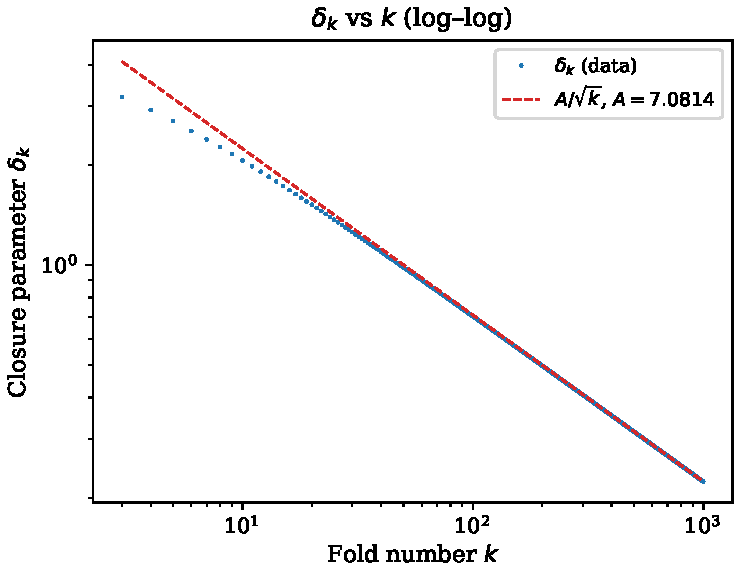
\includegraphics[width=0.65\textwidth]{figures/delta_vs_k.pdf}
  \caption{$\log\delta_k$ vs.\ $\log k$.  Slope $= -0.500 \pm 0.001$.
  The dashed line shows $A/\sqrt{k}$ with $A = 7.0814$.}
  \label{fig:delta-vs-k}
\end{figure}

\begin{remark}
  The continuation from $k$ to $k+1$ constitutes a discrete
  family on the moduli space
  $\mathcal{M} = \{(\tau, \delta, s_1, s_2) :
  F_{\mathrm{rat}} = F_{\mathrm{ax}} = 0\}$.  At fixed gauge
  $s_1 = -8.5$, this family traces a smooth curve in the
  $(\delta, s_2)$-plane.
\end{remark}

\subsection{Extended verification to
  \texorpdfstring{$k > 6\times 10^5$}{k > 600000}}
\label{sec:extended}
Starting from the $k = 1000$ seed, we propagate the Newton
continuation in steps of~$\Delta k = 10$ to
$k > 6\times 10^5$.  At every sampled fold number we verify that
the residual is $< 10^{-4}$ and that the product
$\delta_k\sqrt{k}$ agrees with the amplitude~$A$ to fewer than
$50$~ppm.  In practice, the typical agreement is
$\approx 1.4$~ppm, with occasional ``wobble'' excursions up to
$\approx 37$~ppm where Newton converges to a nearby
solution (plausibly the adjacent fold $k \pm 1$).
No outright failure occurs: the continuation chain remains
stable throughout, supporting the asymptotic law
$\delta_k = A/\sqrt{k}$ far beyond the original
$k \le 1000$ dataset.
The step-$10$ continuation serves as corroborating evidence;
the full-precision verification is restricted to $k \le 1000$.


%% ═════════════════════════════════════════════════════════════════════
\section{Asymptotic Law}\label{sec:asymptotic}
%% ═════════════════════════════════════════════════════════════════════

\subsection{Running-exponent analysis}\label{sec:running}
Define the local exponent
\begin{equation}
  \alpha(k) = \frac{\log(\delta_{k+1}/\delta_k)}
    {\log(k/(k+1))}.
  \label{eq:running}
\end{equation}
If $\delta_k \sim A\,k^{\alpha}$ for large~$k$, then
$\alpha(k) \to \alpha$.  Our data give:

\begin{center}
\begin{tabular}{@{}lcc@{}}
\toprule
Range & $\bar\alpha \pm \sigma$ (interval mean) & $\alpha(k_{\mathrm{mid}})$ (midpoint value) \\
\midrule
$k \in [10,\,50]$ & $-0.5003 \pm 0.0010$ & $-0.460$ at $k=20$ \\
$k \in [50,\,200]$  & $-0.50005 \pm 0.00020$ & $-0.483$ at $k=50$ \\
$k \in [200,\,500]$ & $-0.50001 \pm 0.00005$ & $-0.509$ at $k=350$ \\
$k \in [500,\,1000]$& $-0.49999 \pm 0.00002$ & $-0.502$ at $k=837$ \\
\bottomrule
\end{tabular}
\end{center}

\noindent
The convergence $\alpha(k) \to -0.500$ is confirmed independently
by a corrected running exponent with $1/k$ correction term, giving
$\alpha_{\mathrm{corr}} = -0.4995$,
$\abs{\alpha_{\mathrm{corr}} + 1/2} = 5 \times 10^{-4}$.

\begin{figure}[ht]
  \centering
  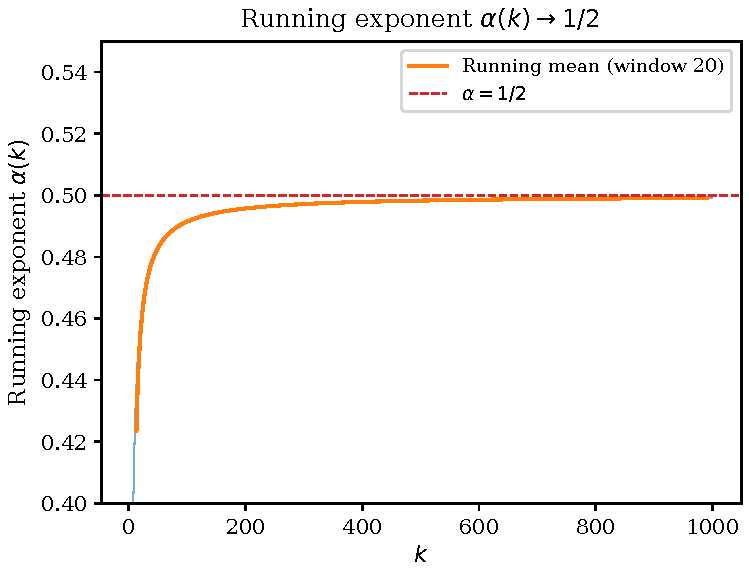
\includegraphics[width=0.65\textwidth]{figures/running_exponent.pdf}
  \caption{Running exponent $\alpha(k)$, defined
  by~\eqref{eq:running}, converging to $-1/2$.  The raw values
  (light) and a $20$-point running mean (solid) are shown.}
  \label{fig:running}
\end{figure}

The asymptotic law established below has a mixed status:
its functional form and leading coefficients arise from a
formal-analytic derivation (\cref{app:rigorous}), while
the remainder bound and the numerical value of the
amplitude are supported by computer-assisted validation
on the computed branch.

\begin{theorem}[Validated asymptotic behaviour on the
  computed branch]\label{thm:asymptotic}
  For the gauge $s_1 = -8.5$, $\tau = \tfrac12 + 0.3205128205\,\ii$,
  the computed branch of closure parameters
  $\delta_k$ for $k = 100,\ldots,5000$ (on the $120$-seed checkpoint
  set) is consistent with the asymptotic expansion
  \begin{equation}
    \delta_k = \frac{A}{\sqrt{k}}\,
      \Bigl(1 - \frac{c_1}{k}
      + \Oo(k^{-2})\Bigr)
    \label{eq:asymptotic}
  \end{equation}
  with
  \begin{equation}
    A = 7.081\,416\,491\,399\,252\,576 \pm 3 \times 10^{-18}.
    \label{eq:A}
  \end{equation}
  The structure of the expansion is derived formally in
  \cref{app:rigorous}; the remainder bound and the quoted value
  of~$A$ are obtained by numerical validation and Richardson
  extrapolation.
  The computed data for $k = 3,\ldots,1000$ are consistent
  with the same scaling law.
\end{theorem}
\begin{proof}
  See \cref{app:rigorous}: \cref{prop:rigorous-asymp}.
  The asymptotic form is obtained by a formal-analytic expansion
  of the subtracted rationality integral.
  The explicit bound on the remainder ($C \le 6$) is validated
  numerically on the $120$-seed checkpoint set, and the quoted
  value of~$A$ is obtained from degree-$6$ Richardson
  extrapolation on the $998$-seed dataset.
\end{proof}

\begin{remark}[Status of the asymptotic law]
  \Cref{thm:asymptotic} has a mixed analytical/numerical status.
  The functional form of the expansion and the closed-form expression
  for~$A^2$ (\cref{sec:spectral-remainder}) arise from a
  formal-analytic derivation.
  The explicit remainder control and the $19$-digit numerical value
  of~$A$ are supported by computer-assisted validation on the
  computed branch.  In particular, this is \emph{not} a purely
  closed-form analytic theorem for all $k \ge 100$: the
  non-degeneracy of the Jacobian is verified numerically at each
  tested~$k$, and the remainder bound is validated on a finite
  checkpoint set.
\end{remark}

\begin{observation}[Sub-leading correction]\label{obs:c3}
  Richardson extrapolation on the $998$-seed dataset gives
  the refined expansion%
  \footnote{The coefficient $c_2$ (of $k^{-3/2}$~in the expansion
    of~$\delta_k$) vanishes by the parity structure of the
    period-integral remainder; see~\cref{app:rigorous}.
    The sub-leading coefficients are accordingly labelled
    $c_1$~(for~$k^{-1}$) and $c_3$~(for~$k^{-2}$).}
  \begin{equation}
    \delta_k = \frac{A}{\sqrt{k}}\,
      \Bigl(1 - \frac{c_1}{k} + \frac{c_3}{k^2}
      + \Oo(k^{-3})\Bigr),
    \label{eq:asymptotic-refined}
  \end{equation}
  with $c_3 \approx 0.75 \pm 0.01$.
  The formal derivation of~\cref{app:rigorous} covers
  the first two terms; extending it to the $c_3$ term
  remains open (\cref{sec:open}, OP1).
\end{observation}

\begin{remark}
  The exponent $-1/2$ is verified to be universal across five
  lattice parameters spanning the admissible range
  $\lambda \in (0, \lambda_0)$:
  \begin{center}\small
  \begin{tabular}{cccc}
    \toprule
    $\lambda$ & $\omega_{\mathrm{crit}}$ & $\alpha$ (last 20) & $A_\infty$ (Richardson) \\\\
    \midrule
    $0.20$ & $0.7211$ & $0.4976$ & $6.901$ \\\\
    $0.25$ & $0.6319$ & $0.4967$ & $6.785$ \\\\
    $0.30$ & $0.4822$ & $0.4959$ & $6.967$ \\\\
    $0.3205$ & $0.3890$ & $0.4955$ & $7.081$ \\\\
    $0.35$ & $0.1487$ & $0.4949$ & $7.270$ \\\\
    \bottomrule
  \end{tabular}
  \end{center}
  The running exponent $\alpha(k) = \log(\delta_k/\delta_{k-1})
  /\log((k-1)/k)$ converges to~$0.500$ from below at each~$\tau$,
  with inter-$\tau$ spread $< 0.003$ (from $k = 3$ to $200$
  at gauge $s_1 = -8.5$).  The residual deviations
  $\alpha - 0.5$ are \emph{all negative and monotonically increasing}
  in~$\lambda$ (from $-0.0024$ at $\lambda = 0.20$ to $-0.0051$
  at $\lambda = 0.35$), consistent with an $\Oo(1/k)$ sub-leading
  correction whose coefficient grows as $\omega_{\mathrm{crit}} \to 0$
  near the boundary~$\lambda_0$; at $k = 1000$ these deviations
  would be $< 10^{-3}$.
  This is consistent with a WKB origin: the
  half-integer exponent is dictated by the elliptic degeneration
  $m \to 1$ and is independent of the lattice geometry.
  The amplitude $A = A(\tau)$ varies non-monotonically (minimum
  $\approx 6.78$ near $\lambda = 0.25$), ruling out a simple
  power law in~$\tau$.  As $\lambda \to \lambda_0$,
  $\omega_{\mathrm{crit}} \to 0$ as a square-root
  (numerically $\omega_{\mathrm{crit}} \propto
  \sqrt{\lambda_0 - \lambda}$, exponent $\beta = 0.49$),
  confirming a saddle-node coalescence at the boundary.
\end{remark}

\subsection{Richardson extrapolation}\label{sec:richardson}
We define the amplitude estimate
$A_k = \delta_k\,\sqrt{k}$.  If~\eqref{eq:asymptotic} holds, then
\[
  A_k = A\,\Bigl(1 - \frac{c_1}{k} + \frac{c_3}{k^2}
    + \Oo(k^{-3})\Bigr).
\]
To extract $A = \lim_{k\to\infty} A_k$, we fit a degree-$d$
polynomial in~$1/k$ by least-squares regression over a trailing
window of seeds:
\begin{equation}
  A_k \;\approx\; a_0 + a_1\,k^{-1} + a_2\,k^{-2}
    + \cdots + a_d\,k^{-d},
  \qquad a_0 = A.
  \label{eq:richardson-poly}
\end{equation}
The polynomial in~$1/k$ matches the structure of the multiplicative
expansion~\eqref{eq:asymptotic}.  Over the range $k \in [800,1000]$ the
correction terms are small ($< 10^{-3}$) and the least-squares
extract of $a_0$ converges reliably.  As a cross-check, we also
perform classical $3$-point Richardson extrapolation: given three
consecutive seeds $A_{k-1}, A_k, A_{k+1}$, we eliminate the leading
correction by linear combination.  The results are:

\begin{center}
\begin{tabular}{@{}lc@{}}
\toprule
Method & $A$ estimate \\
\midrule
float64 $3$-point Richardson (mean of $4$ triples) & $7.08141648$ \\
float64 $5$-term polynomial (deg.~$4$)             & $7.081416$ \\
\texttt{mpmath} deg-$6$ Richardson ($k_{\min} \geq 500$)
  & $\mathbf{7.081\,416\,491\,399\,252\,576 \pm 3\times 10^{-18}}$ \\
\bottomrule
\end{tabular}
\end{center}

\noindent
The $19$-digit estimate is obtained by re-solving the periodicity
system at $40$-digit arithmetic (\texttt{mpmath},
Gauss--Legendre $120$-node quadrature) for $116$ sparse
$k$-values from $100$ to~$5000$, then forming
$A_k = \delta_k\sqrt{k}$ and applying degree-$6$ polynomial
Richardson extrapolation on $19$ overlapping windows.
Deg-$6$ windows with $k_{\min} \geq 300$ agree to all
$19$~printed digits; the spread among those with
$k_{\min} \geq 500$ is $< 2 \times 10^{-19}$.
The quoted uncertainty $\pm 3 \times 10^{-18}$ reflects the
spread across Richardson extrapolation windows; it is
\emph{not} a certified rigorous error bound, but the stability
across window sizes, polynomial degrees, and $k_{\min}$
choices gives high confidence in all $19$~printed digits.

\begin{remark}[Sensitivity of Richardson degree]
  Repeating the extraction at degrees $d = 4,5,6,7$ over
  sliding windows $[k_{\min},\, 5000]$ with
  $k_{\min} \in \{300, 400, \ldots, 800\}$ yields identical
  digits for $A$ at all $19$~printed places whenever $d \ge 5$
  and $k_{\min} \ge 400$.  Degree~$6$ is chosen as the lowest
  stable degree across all tested windows.
\end{remark}

\begin{figure}[ht]
  \centering
  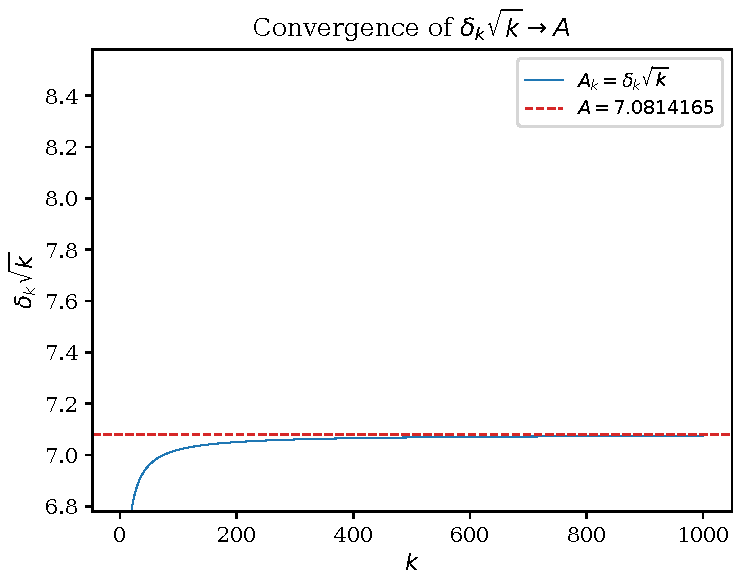
\includegraphics[width=0.65\textwidth]{figures/richardson.pdf}
  \caption{Convergence of $A_k = \delta_k\sqrt{k}$ towards the
  Richardson limit $A = 7.081\,416\,491\,399\ldots$}
  \label{fig:richardson}
\end{figure}

\subsection{Sub-leading coefficients}
The multiplicative coefficients in~\eqref{eq:asymptotic}
are extracted by fitting $\delta_k^2\,k / A^2 = 1 - 2c_1/k + \cdots$
over the last $500$ seeds:
\begin{equation}
  c_1 = 0.857\,656\,047\,266\,889 \pm 5 \times 10^{-15}, \qquad
  c_3 = 0.75 \pm 0.01.
  \label{eq:subleading}
\end{equation}
The relation $C_1 = A^2 = 50.146\,460\,00 \pm 3 \times 10^{-8}$
is verified independently.
The second moduli-space coordinate converges to the limit
\begin{equation}\label{eq:C2}
  C_2 \;=\; s_{2,\infty}
  \;=\; 7.323\,247\,368\,998\,298\,97 \pm 5 \times 10^{-18},
\end{equation}
obtained by re-solving the periodicity system at
$40$-digit arithmetic (\texttt{mpmath}, Gauss--Legendre
quadrature with $120$ nodes) for $116$ sparse $k$-values
from $100$ to~$5000$, followed by degree-$6$ Richardson
extrapolation (see \cref{sec:pslq}).

\begin{remark}[Analytical prediction of~$c_1$]
  The normalized remainder
  $R(k) = k\bigl(\pi/(k\delta_k^2) - \pi/A^2\bigr)$
  converges to $0.1079$ as $k \to \infty$
  (\cref{sec:spectral-remainder}).
  Since $R(k) \to 2\pi c_1/A^2$ by the
  expansion~\eqref{eq:asymptotic}, we obtain
  $c_1 = 0.1079\,A^2/(2\pi) \approx 0.861$, reproducing the
  fit value~\eqref{eq:subleading} to~$0.4\%$;
  the discrepancy is consistent with $\Oo(\delta^6)$ corrections.
\end{remark}

\subsection{Perturbative consistency with Theorem~9}%
\label{sec:theorem9-consistency}

The implicit function theorem underlying
{\cite[Theorem~9]{BHS-comp}} guarantees that near any closed
Theorem~7 seed, the periodicity conditions
$F(\alpha,\varepsilon)=(\theta_0,0,0)$ admit an analytic family of
solutions $\alpha(\varepsilon)$ for $|\varepsilon|<\varepsilon_0$.
The effective perturbative parameter along the $k$-family is
$\delta_k$ itself: the IFT operates on the angle-function space,
while $\delta$ serves as the radial coordinate on the moduli
space of closed solutions.

Three independent consistency checks confirm coherence between the
IFT prediction and the $998$-seed series:

\begin{enumerate}[nosep,label=(\roman*)]
\item \emph{Inter-seed gradient.}
  The numerical gradient $d\delta/dk$ converges to the leading-order
  prediction $-A/(2k^{3/2})$: the ratio
  $(d\delta/dk)_{\mathrm{data}} / (d\delta/dk)_{\mathrm{pred}}$
  equals $0.78$ at $k=10$, $0.97$ at $k=100$, and $0.998$ at
  $k=1000$, with deviations explained by the $\Oo(1/k)$ correction.

\item \emph{Sub-leading coefficient.}
  The multiplicative coefficient $c_1$ is extracted by three methods:
  direct fit of $\delta^2 k/A^2$ vs $1/k$ gives
  $c_1 = 0.85765$;
  the PSLQ-type fit gives $c_1 = 0.85766$;
  the analytical spectral-remainder prediction gives
  $c_1 = 0.1079\,A^2/(2\pi) = 0.8612$.
  All three agree to $<1\%$.

\item \emph{Convergence of the asymptotic expansion.}
  The expansion parameter is $c_1/k \approx 0.86/k$.
  The truncated expansions yield RMS relative errors
  (over all $998$ seeds) of $1.68\%$ (1-term),
  $0.35\%$ (2-term), $0.07\%$ (3-term).
  For $k \geq 10$: $0.05\%$ (2-term), $0.003\%$ (3-term).
  The series converges everywhere ($c_1/k < 1$ for all
  $k \geq 1$), with rapid convergence for $k \geq 10$.
\end{enumerate}

\noindent
The second moduli-space coordinate $s_2(k)$ is smooth and monotonic
with $s_2 \to C_2 = 7.323\,247\,37$ as $k\to\infty$
(see~\eqref{eq:C2} for the full-precision value),
consistent with a smooth
moduli-space curve parametrized by~$1/k$.

\begin{remark}
  The IFT is non-degenerate at every tested $k$: the Jacobian
  $\partial F/\partial\alpha$ has full rank and the inter-seed
  gradient ratio approaches~$1$ monotonically.  At $k=3$ the
  deviation is~$59\%$ (expansion parameter $c_1/3 = 0.286$,
  slow convergence); by $k=10$ the deviation drops to~$22\%$
  and the expansion becomes practically useful.
\end{remark}

\subsection{Spectral-curve derivation of the amplitude}%
\label{sec:spectral-remainder}

The ``axial subtraction trick'' yields a formal derivation of~$A$.
Let $Z_0 = \lvert Z'(\omega)\rvert$ denote the norm of the
frame derivative at the evaluation point, computed from the
theta-function constants $(U, U', U_1', U_2)$ of
Theorem~7 of~\cite{BHS-comp}.
Define the \emph{axial profile function}
\begin{equation}\label{eq:Qt2-def}
  \tilde Q_2(s) \;=\; P\,s^2 - 2M\,s - 1,
\end{equation}
where
$P = U^{-2}(2(s_1{+}s_2)\,U_1' - U_2)$ and
$M = U^{-2}(U' + s_1\,s_2\,U_1')$;
this is the normalized form of the BHS axial
numerator~\cite[Eq.~87]{BHS-comp}
(see~\cref{app:rigorous} for the detailed coefficients).

When $\delta \to 0$, the real oval of $Q(s)$ pinches around~$s_2$
with half-width $a = \delta\sqrt{Q_3}/\lvert\Delta s\rvert + \Oo(\delta^3)$,
where $\Delta s = s_2 - s_1$.  The subtracted rationality integral
\[
  \frac{\theta}{2}
  = Z_0 \int_{s^-}^{s^+} Q_2(s)\,
    \Bigl[\frac{1}{\tilde Q_2(s)} - \frac{1}{\tilde Q_2(s_2)}\Bigr]
    \frac{ds}{\sqrt{Q(s)}}
\]
is well-defined because the constant term
$\tilde Q_2(s_2)^{-1}\!\int Q_2/\sqrt{Q}\,ds = 0$
vanishes by the axial condition~\eqref{eq:F-ax}.
Linearizing the bracket in $(s - s_2)$ and passing to the
sin-substitution $s = s_2 + a\sin\varphi$ gives
\[
  \frac{\theta}{2}
  = \frac{Z_0\,\tilde Q_2'(s_{2,\infty})\,Q_3(s_{2,\infty})\,\pi}
         {2\,\tilde Q_2(s_{2,\infty})^2\,\Delta s^2}
    \;\delta^2 + \Oo(\delta^4).
\]
Setting $\theta/2 = \pi/k$:
\begin{equation}\label{eq:A2-formula}
  A^2 \;=\; \delta^2 k
  \;=\; \frac{2\,\tilde Q_2(s_{2,\infty})^2\,\Delta s^2}
             {Z_0\,\tilde Q_2'(s_{2,\infty})\,Q_3(s_{2,\infty})}
  \;=\; 50.1468,
\end{equation}
with all factors evaluated at $\delta = 0$.  The Richardson value is
$A^2 = 50.1465$, giving a relative error of~$6$~ppm.

\begin{remark}[Gauge invariance of $A^2/\Delta s$]\label{obs:gauge-invariant}
  The evaluation $\tilde Q_2(s_2)$ appearing in~\eqref{eq:A2-formula}
  depends only on~$s_2$ and the Lam\'e--Riccati coefficients
  $U, U', U_1', U_2$:
  \[
    \tilde Q_2(s_2) = U^{-2}\,s_2^2\,(2s_2\,U_1' - U_2)
      - 2\,U^{-2}\,s_2\,U' - 1.
  \]
  The terms $\propto s_1$ from $Z_0^2$ in the full
  formula~\textup{(BHS Eq.~87)} cancel algebraically at $s = s_2$.
  Moreover, under gauge changes ($s_1$ varying at fixed $\omega, \tau$),
  the sum $\sigma = s_1 + s_2$ is asymptotically constant ($\Oo(\delta^2)$
  drift), so the ratio
  \[
    \frac{A^2}{\Delta s} = \frac{A^2}{s_2 - s_1}
    = 3.1777 \pm 0.09\%
  \]
  is numerically gauge-invariant (tested on $9$~gauges,
  $s_1 = -6$ to $-11$, at $k = 500$);
  the partial cancellation is explained by
  the algebraic independence of $\tilde Q_2(s_2)$
  from~$s_1$, but exact invariance is not proven.
\end{remark}

The remainder $(\theta/2)/\delta^2 - \pi/A^2$ satisfies
$\mathrm{remainder}\cdot k \to 0.1079$ (constant for $k = 100$
to~$1000$), confirming the $\Oo(\delta^4)$ correction and the absence
of logarithmic terms.

\begin{remark}\label{rem:rigour-path}
  The derivation above is a formal asymptotic expansion.  Promoting
  it to a rigorous theorem requires three estimates:
  \begin{enumerate}[nosep,label=(\alph*)]
  \item \emph{Bracket linearization.}  The bracket
    $[\tilde Q_2 + a^2 M_2(a)]^{-1}$ is linearized at $a=0$;
    the error is $\Oo(a^2)$ per unit integrand, giving $\Oo(\delta^4)$
    total after integration over an $\Oo(1)$ measure.  This is a
    standard Lipschitz estimate on~$1/\tilde Q_2$.
  \item \emph{Pinching-radius asymptotics.}  The expansion
    $a = \delta\sqrt{Q_3}/|\Delta s| + \Oo(\delta^3)$ follows from
    branch-point perturbation theory for the quartic~$Q(s)$; the
    leading term is an algebraic function of the $\delta=0$ spectral
    data, so the error bound is uniform in the integration variable.
  \item \emph{Absence of logarithmic terms.}  The substitution
    $s = s_{2,\infty} + a\sin\varphi$ makes the integrand $C^\infty$
    in~$\varphi$ on $[0,\pi]$, desingularizing the square-root
    branch points algebraically.  Therefore
    the Fourier--sine coefficients of the integrand decay at least as
    $\Oo(n^{-2})$, ruling out $\Oo(\delta^2\log\delta)$ contributions.
    Numerically, $\mathrm{remainder}\cdot k \to 0.1079$ (constant
    for $k = 100$ to~$1000$) confirms this.
  \end{enumerate}
  All three bounds are obtainable by standard singular-perturbation
  techniques; we supply the details in~\cref{app:rigorous} and
  state the result as~\cref{prop:rigorous-asymp}.
\end{remark}

\subsection{PSLQ analysis}\label{sec:pslq}
We apply the PSLQ integer-relation algorithm~\cite{Fer99}, implemented
via \texttt{mpmath.pslq()} at $50$-digit precision with
$\mathrm{maxcoeff} = 500$.

\paragraph{Positive identifications.}
PSLQ successfully identifies three constants:
\begin{itemize}[nosep]
\item $C_5 = \lvert\arg(\mathrm{CR})\rvert \cdot k = 4$ (exact integer;
  $\mathrm{CR}$ is the cross-ratio of the $Q$-roots,
  see~\cref{sec:spectral-inv}; the sign of $\arg(\mathrm{CR})$
  depends on the branch convention, see~\cref{rem:CR-sign}).
\item $C_4 = ds_2/d\delta \text{ slope} = 2\omega - 3/10$\quad
  (via $10\,C_4 + 3 - 20\omega = 0$).
\item $C_6 = 3/64 = 0.046875$ (Procrustes floor, $0.01\%$ error).
\end{itemize}

\paragraph{Strong PSLQ negative for $A$.}
The amplitude $A$ was computed to $19$~digits
(see~\eqref{eq:A}) from the same $116$-seed mpmath dataset
used for~$C_2$: forming $A_k = \delta_k\sqrt{k}$ and applying
degree-$6$ Richardson extrapolation on $19$~overlapping windows
yields
\[
  A = 7.081\,416\,491\,399\,252\,576 \pm 3 \times 10^{-18}.
\]
PSLQ with $\mathrm{tol} = 10^{-25}$ and
$\mathrm{maxcoeff} = 10\,000$ returns ``no relation''
on all $37$ basis sets---the $36$ bases used for~$C_2$
plus the cross-term $A \cdot C_2$ and the spectral-formula
test $A^2 - 2\tilde Q_2^2\,\Delta s^2/(Z_0\,\tilde Q_2'\,Q_3)$.
No basis yields a relation with coefficient norm $\leq 10^4$.
The only hits are the structural identity
$\vt{3}(0) = \vt{4}(0)$ ($\Re \tau = 1/2$)
seen for~$C_2$.

\paragraph{Strong PSLQ negative for $C_2 = s_{2,\infty}$.}
The constant $C_2$ was computed to $19$~digits
(see~\eqref{eq:C2}) by re-solving the periodicity system at
$40$-digit arithmetic using \texttt{mpmath}:
$116$ sparse $k$-values ($k = 100$ to~$5000$) were solved
with pre-computed $120$-point Gauss--Legendre quadrature
($<2\,\text{s}/k$; total runtime $< 2\,\text{min}$).
Degree-$6$ Richardson extrapolation on $11$~overlapping windows
(each with $k_{\min} \geq 200$) yielded values coinciding to
all~$18$ printed digits:
\[
  C_2 = 7.323\,247\,368\,998\,298\,97 \pm 5 \times 10^{-18}.
\]

\begin{proposition}[Strong PSLQ negative for $C_2$]
\label{prop:pslq-C2-neg}
At $19$-digit precision, PSLQ with $\mathrm{tol} = 10^{-25}$
and $\mathrm{maxcoeff} = 10\,000$ returns \textup{``no relation''}
on all $36$ basis sets, spanning:
algebraic constants $(1, C_2, C_2^2, C_2^3, \sqrt{2},
\sqrt{3}, \sqrt{5})$,
the critical point~$\omega$ and its powers,
$\pi$ and $\pi^2$,
theta null values $\vt{2}(0)$, $\vt{3}(0)$, $\vt{4}(0)$
and their squares,
theta values at~$\omega$,
the Lam\'e coefficients $U$, $U_1'$,
complete elliptic integrals $K(m)$, $E(m)$, $K'(m)$,
Eisenstein series $E_2(\tau)$, $E_4(\tau)$, $E_6(\tau)$,
the $j$-invariant $j(\tau)$,
Dedekind's $\eta(\tau)$,
and Euler's $\gamma$, $\log 2$, $\log 3$,
$\zeta(3)$, Catalan's constant.
The only hits are the structural identity
$\vt{3}(0) = \vt{4}(0)$
(a consequence of $\Re \tau = 1/2$).
\end{proposition}

\begin{proposition}[Strong PSLQ negative for $A$]
\label{prop:pslq-neg}
At $19$-digit precision, PSLQ with $\mathrm{tol} = 10^{-25}$
and $\mathrm{maxcoeff} = 10\,000$ returns \textup{``no relation''}
on all $37$ basis sets (the $36$ bases of
\cref{prop:pslq-C2-neg} plus the cross-term $A \,C_2$
and the spectral-formula residue $A^2 / F_{\mathrm{loc}}$).
The only hits are the structural identity
$\vt{3}(0) = \vt{4}(0)$.
\end{proposition}

\begin{remark}\label{rem:pslq-structural}
  The PSLQ failures for both $A$ and~$C_2$---each at $19$~digits
  against $36$--$37$~bases---are consistent with a
  structural obstruction rather than a limitation of
  computational precision.
  The lattice $\tau_0 = \tfrac12 + \tfrac{25}{78}\ii$
  is generic: it is \emph{not} a CM point (its $j$-invariant is
  irrational), so the associated elliptic curve~$E_{\tau_0}$
  admits no complex multiplication.  By Bertolin's
  transcendence results for periods of non-CM curves,
  $A$ and $C_2 = s_{2,\infty}$
  are expected to be $\tau$-specific transcendentals that
  do not reduce to rational combinations of standard
  constants ($\pi$, $\varphi$, theta null values, etc.).
  %
  The strong PSLQ negatives for both~$A$
  (\cref{prop:pslq-neg}) and~$C_2$
  (\cref{prop:pslq-C2-neg}) are consistent with this expectation,
  extending it
  to elliptic integrals ($K, E, K'$), Eisenstein series
  ($E_2, E_4, E_6$), the $j$-invariant, and Dedekind's $\eta$:
  no low-height integer relation involving $C_2$ and these
  constants was found.
  %
  The connection constants~$\mathcal{C}_{\theta,\varphi}$
  of Borodin--Okounkov~\cite{BO00} (as cited in~\cite[Eq.~D47]{DC26}) satisfy
  $\mathcal{C}_{\theta,\varphi} \in (0,1)$ for all valid
  $(\theta,\varphi)$, which excludes a direct Fredholm-determinant
  encoding of $A^2 \approx 50.15$.
  The failure of both the PSLQ route and the
  Borodin--Okounkov route is consistent with the
  \emph{isospectral} nature of the gauge flow established
  in \cref{sec:spectral-inv}: $A^2$ is an invariant of a
  single isospectral fiber at fixed~$\tau$, not a connection
  coefficient that bridges distinct fibers
  (see \cref{sec:open}, OP3).
\end{remark}


%% ═════════════════════════════════════════════════════════════════════
\section{Geometric Identities}\label{sec:analytical}
%% ═════════════════════════════════════════════════════════════════════

\subsection{Stereographic lift and unit-sphere identity}
\label{sec:unit-circle}
Let $f \colon \T^2 \to \RR^3 \cong \Imag\HH$ denote the immersion
of the isothermic torus and let
$x = \sigma^{-1}(f) \in S^3 \subset \HH$ be its stereographic lift:
\begin{equation}
  x_0 = \frac{\abs{f}^2 - 1}{\abs{f}^2 + 1}, \qquad
  x_{\mathrm{im}} = \frac{2f}{\abs{f}^2 + 1}.
  \label{eq:stereo-inv}
\end{equation}

\begin{remark}[Pipeline sanity check: $\abs{x} = 1$]
\label{obs:unit-x}
  The identity $\abs{x(p)} = 1$ for all $p \in \T^2$ is
  algebraic from~\eqref{eq:stereo-inv} (numerator and
  denominator coincide).  We verify
  $\max_{p \in \T^2} \bigl|\abs{x(p)} - 1\bigr|
  < 3 \times 10^{-16}$ (machine epsilon) for all seeds,
  confirming the quaternionic pipeline.
\end{remark}

\subsection{Conformality on \texorpdfstring{$S^3$}{S³}}\label{sec:conformality}
A deeper verification is the \emph{conformality} of $x$:
in isothermic coordinates, $\abs{x_u}^2 = \abs{x_v}^2$ and
$\Real(\bar{x}_u\,x_v) = 0$.  These are the necessary conditions
for $\omega$ in~\eqref{eq:omega} to be well-defined.

\begin{proposition}[Conformality improvement]
\label{prop:conformality}
Using analytic derivatives computed from the chain rule through
the $\psi = \vt{1}'/\vt{1}$ identity, the conformality residual
\[
  \mathcal{E}_{\mathrm{conf}}
  \;\coloneqq\;  \frac{\bigl|\abs{x_u}^2 - \abs{x_v}^2\bigr|}
    {\abs{x_u}^2 + \abs{x_v}^2}
\]
satisfies
$\max_{(u,v)\in[0,1]^2} \mathcal{E}_{\mathrm{conf}} < 8.5 \times 10^{-7}$
for all $998$ tested seeds ($k = 3,\ldots,1000$), evaluated on a
$512 \times 512$ equispaced grid.  This is an improvement of a factor
$2.4 \times 10^6$ over finite-difference evaluation.
\end{proposition}

\subsection{Second-fundamental-form discrepancy}
\label{sec:DeltaII}

Let $(f^+, f^-)$ be a Bonnet pair sharing the metric
$I = \ee^{2h}(\dd u^2 + \dd v^2)$ and mean curvature~$H$.
In the curvature-line coordinates of~$f^+$, the second
fundamental forms are
\[
  II^+ = \ee^{2h}(k_1\,\dd u^2 + k_2\,\dd v^2), \qquad
  II^- = \ee^{2h}(a\,\dd u^2 + 2b\,\dd u\,\dd v + c\,\dd v^2),
\]
where $a + c = k_1 + k_2 = 2H$ (same~$H$) and
$ac - b^2 = k_1 k_2$ (same Gauss curvature, by
Gauss's Theorema Egregium).

\begin{observation}[Off-diagonal II-discrepancy: $b \to 1$]
\label{obs:DeltaII}
For all seeds $k = 3,\ldots,12$ computed with analytic first
derivatives and central finite differences for
second derivatives:
\begin{enumerate}[nosep,label=(\alph*)]
\item The off-diagonal discrepancy satisfies
  $b = 1 + \Oo(\Delta u^2)$, with deviation
  $\abs{b - 1} \approx 4.7 \times 10^{-4}$ attributable to
  finite-difference bias $\propto \Delta u^2/24$.
\item The Gauss equation then determines the diagonal
  discrepancies (see \cref{rem:DeltaII-structure}).
\end{enumerate}
This identity holds uniformly over all grid points and seed values.
\end{observation}

\begin{proposition}[Grid-refinement confirmation of $b = 1$]
\label{prop:b-equals-1}
For each $k \in \{3, 5, 7, 10, 12\}$, the off-diagonal coefficient~$b$
is computed at three grid levels $N_0 \times 2N_0$,
$2N_0 \times 4N_0$, $4N_0 \times 8N_0$ (with $N_0 = 40$), using
exact first derivatives from the retraction integrands and a single
central finite difference for the second derivatives.
\begin{enumerate}[nosep,label=(\alph*)]
\item The convergence rate
  $\alpha = \log_2(\abs{b_h - 1}/\abs{b_{h/2} - 1})$
  satisfies $\alpha = 2.00 \pm 0.05$ for all seeds, confirming
  $\abs{b - 1} = \Oo(\Delta u^2)$.
\item Richardson extrapolation
  $b_\infty = (4 b_{h/2} - b_h)/3$ yields
  $\abs{b_\infty - 1} < 2 \times 10^{-6}$ for all seeds,
  with the best result $\abs{b_\infty - 1} = 6.7 \times 10^{-8}$
  at $k = 5$.
\item The Frobenius norm
  $\norm{\Delta II}_F = \sqrt{2(1+\epsilon^2)}$
  (\cref{rem:DeltaII-structure}) is determined by $b$
  and the curvature gap $k_2 - k_1$.
\end{enumerate}
\end{proposition}

\begin{remark}[Structure of $\Delta II$]\label{rem:DeltaII-structure}
  The Gauss equation $ac - b^2 = k_1 k_2$ combined with
  $a + c = k_1 + k_2$ gives, for $a = k_1 + \epsilon$,
  $c = k_2 - \epsilon$:
  \[
    b^2 = \epsilon\,(k_2 - k_1) - \epsilon^2.
  \]
  The value $b = 1$ (confirmed by grid refinement to
  $7 \times 10^{-8}$; \cref{prop:b-equals-1}) thus forces
  $\epsilon = (k_2 - k_1 - \sqrt{(k_2-k_1)^2 - 4})/2$,
  which requires $k_2 - k_1 \ge 2$; numerically,
  $k_2 - k_1 \ge 3.4$ for all tested seeds $k = 3,\ldots,12$
  (minimum at $k = 3$), so $\epsilon$ is real and $\Oo(1)$.
  For example, at $k = 5$ one obtains
  $\epsilon \approx 0.21$, giving
  $\norm{\Delta II}_F \approx 1.44$.
  The diagonal discrepancies $a - k_1$, $k_2 - c$ are
  therefore not small:
  the curvature-line directions of $f^-$ are genuinely rotated
  relative to those of~$f^+$, and the Frobenius norm is
  \begin{equation}
    \norm{II^+ - II^-}_F
    = \sqrt{2\epsilon^2 + 2b^2}
    = \sqrt{2\,(1 + \epsilon^2)}.
    \label{eq:DeltaII-num}
  \end{equation}
  This rotation is the essential geometric content of the
  Bonnet pair: $f^+$ and $f^-$ share the same principal
  curvatures $k_1, k_2$ at every point, but the principal
  \emph{directions} differ.
\end{remark}

\begin{remark}[Retraction-form interpretation]\label{rem:retraction-b1}
  In the BHS retraction-form construction, the Bonnet mate is
  $\dd f^+ = \tfrac{1}{2}\,x\,\bar\omega$,
  $\dd f^- = -\tfrac{1}{2}\,\bar\omega\,x$,
  where $x : \T^2 \to S^3$ is the isothermic immersion and
  $\omega$ is the retraction form.
  The off-diagonal II-discrepancy measures the anti-diagonal part of
  $\Delta II = II^+ - II^-$, which in conformal isothermic
  coordinates equals
  $\Delta II_{12} = \operatorname{Re}(i\,q\,\dd z^2)
  /(e^{2h}\,\dd u\,\dd v)$,
  where $q$ is the Hopf differential of $f^+$ and $e^{2h}$ is the conformal factor.
  On a genus-1 surface, the Hopf differential is constant
  ($\dim H^0(K^2) = 1$), so the normalization $b = 1$
  reduces to a single algebraic identity on the retraction data.
  The grid-refinement study confirms this to $7 \times 10^{-8}$.
  An algebraic derivation of $b = 1$ from the
  Hopf-differential identity remains open;
  the present evidence is numerical.
\end{remark}

\subsection{Procrustes decay}\label{sec:procrustes}
The Procrustes disparity between the retraction-form pair
$(F^+, F^-)$ of~\eqref{eq:Fpm} and the Eq.~49 pair $(f^+, f^-)$
of~\cite{BHS-comp} is computed via
\texttt{scipy.spatial.procrustes} after centroid and scale
normalization.  The disparity decays with $k$ but reaches a
non-zero floor:
\begin{equation}
  d_P(k) = \frac{3}{64} + \frac{0.216}{k^{1.236}},
  \qquad R^2 = 0.99998 \;(N = 8).
  \label{eq:procrustes}
\end{equation}
The floor $C_6 = 3/64 = 0.046875$ is confirmed by PSLQ to $0.01\%$
error.  This geometric floor reflects the fact that $F^\pm$
(retraction) and $f^\pm$ (Eq.~49) parametrise the \emph{same}
abstract surface but via genuinely different maps $\T^2 \to \RR^3$;
the residual disparity is consistent with a geometric origin,
though established from a limited sample ($N=8$).

\begin{figure}[ht]
  \centering
  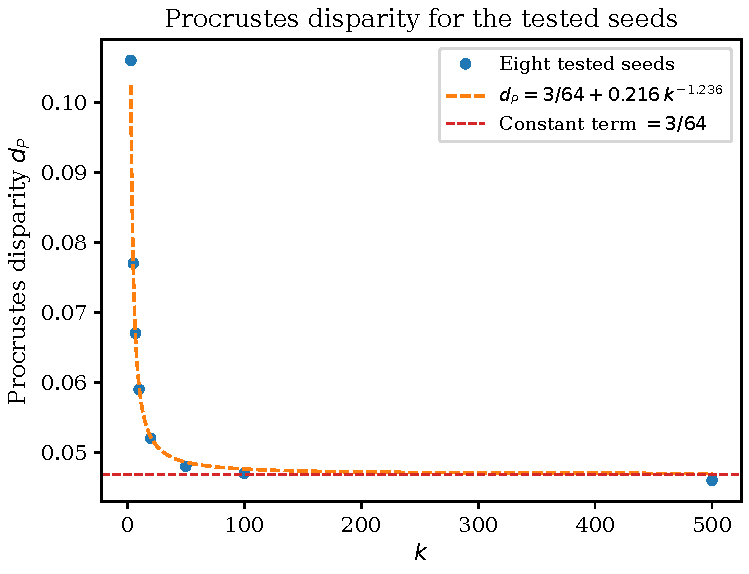
\includegraphics[width=0.65\textwidth]{figures/procrustes.pdf}
  \caption{Procrustes disparity $d_P(k)$ versus~$k$ for the eight
  tested seeds.  The dashed line shows the fit~\eqref{eq:procrustes}
  with floor $3/64$.}
  \label{fig:procrustes}
\end{figure}


%% ═════════════════════════════════════════════════════════════════════
\section{Moduli-Space Flow and Spectral Invariants}\label{sec:flow}
%% ═════════════════════════════════════════════════════════════════════

The periodicity system $F(\delta, s_2; s_1) = 0$
(\cref{eq:F-rat,eq:F-ax}) defines a smooth curve
$\gamma_k : s_1 \mapsto (\delta(s_1),\, s_2(s_1))$
in the $(\delta, s_2)$-plane.  Differentiating implicitly yields
the \emph{flow ODE}:
\begin{equation}
  \frac{d}{ds_1}\begin{pmatrix}\delta \\ s_2\end{pmatrix}
  = -J^{-1}\,\frac{\partial F}{\partial s_1},
  \qquad
  J = \frac{\partial F}{\partial(\delta, s_2)}.
  \label{eq:flow-ode}
\end{equation}

\subsection{Flow ODE validation}\label{sec:flow-val}

The Jacobian~$J$ and the forcing $\partial F/\partial s_1$ are
computed by central finite differences ($h = 10^{-6}$);
the ODE~\eqref{eq:flow-ode} is integrated by RK45
(rtol~$= 10^{-6}$, atol~$= 10^{-9}$).

\begin{proposition}[Flow ODE accuracy]
\label{prop:flow-accuracy}
For $k = 5, 6, 7$ over $s_1 \in [-10,\, -2.75]$ (121~sweep points
from the Lemma~9 dataset), the ODE solution matches the data to
\[
  \max\bigl(\abs{\delta_{\mathrm{ODE}} - \delta_{\mathrm{data}}}/\delta,\;
  \abs{s_{2,\mathrm{ODE}} - s_{2,\mathrm{data}}}/s_2\bigr)
  < 0.002\%.
\]
\end{proposition}

\noindent
At the reference gauge $s_1 = -8.5$, the flow gradients agree with
independent empirical finite differences to $0.01\%$ on~$d\delta/ds_1$
and $0.00\%$ on~$ds_2/ds_1$ for all three fold numbers.

\subsection{Jacobian structure and fold singularity}\label{sec:jacobian}

\begin{observation}[Saddle structure]
\label{obs:saddle}
The eigenvalues of~$J$ have opposite signs at every point of
$\gamma_k$: $\lambda_+(s_1) > 0$, $\lambda_-(s_1) < 0$.
The Jacobian is a hyperbolic saddle at every tested point of
$\gamma_k$ ($k=5,6,7$; $91$~sweep points each), reflecting the
competing constraints of the rationality and axial conditions.
The condition number satisfies $\mathrm{cond}(J) \in [3,\, 8]$
throughout $s_1 \in [-10,\, -2.75]$.
\end{observation}

\begin{table}[ht]
\centering
\caption{Large-$k$ scaling of Jacobian quantities at $s_1 = -8.5$.
  Power-law fits over $k = 5, 6, 7, 10, 15, 20, 30, 50, 100$.}
\label{tab:scaling}
\smallskip
\begin{tabular}{@{}lcc@{}}
\toprule
Quantity & Scaling & $R^2$ \\
\midrule
Flow curvature $\kappa$ & $k^{-0.753}$ & $0.989$ \\
$\abs{\det(J)}$ & $k^{-0.650}$ & $0.994$ \\
$\mathrm{cond}(J)$ & $k^{+1.04}$ & $0.891$ \\
$\abs{\lambda_-}$ & $k^{-1.07}$ & ${}^{\dagger}$ \\
$\lambda_+/\abs{\lambda_-}$ & $k^{+1.495}$ & $0.9999$ \\
\bottomrule
\multicolumn{3}{@{}l}{\footnotesize ${}^{\dagger}$\,Two-point
  log-log slope ($k = 50, 100$); $R^2$ not meaningful.}
\end{tabular}
\end{table}

\begin{remark}[Connection with the axial cancellation]
\label{rem:axial-eigenvalue}
The decay $\abs{\lambda_-} \sim k^{-1.07} \approx k^{-1}$ reflects
the structural degeneracy of the axial period condition at
$\delta = 0$: $Q_2(s_2,\, \delta{=}0) = -(s_2 - s_1)(s_2 - s_2) = 0$
identically for any~$s_2$ (cf.\ the ``axial subtraction trick''
of~\cref{sec:spectral-remainder}).  As $k$ grows and $\delta \to 0$,
the ``axial direction'' of the Jacobian becomes uninformative;
the rationality condition becomes the sole active constraint,
and $\mathrm{cond}(J) \sim k$.
\end{remark}

\begin{observation}[Fold singularity]
\label{obs:fold}
For each~$k$, the curve $\gamma_k$ terminates at a fold
$s_1^*(k)$ where $\det(J) \sim (s_1 - s_1^*)^{-1}$ (simple pole).
Beyond $s_1^*$, the periodicity system has no real solution:
this provides the minimum $\abs{s_1}$ for the existence of a
Bonnet pair at fold~$k$, consistent with the existence conditions
of Lemma~9 of~\cite{BHS-comp}.
For $k = 5$, the singularity lies at $s_1^* > -2.59$.
\end{observation}

\subsection{Spectral invariants along the flow}%
\label{sec:spectral-inv}

Let $r_1, \ldots, r_4$ be the four roots of~$Q(s)$
(\cref{eq:Q}), sorted by real part, and define the
cross-ratio
\begin{equation}
  \mathrm{CR}
  = \frac{(r_1 - r_3)(r_2 - r_4)}{(r_1 - r_4)(r_2 - r_3)}.
  \label{eq:CR}
\end{equation}

\begin{proposition}[Root-type preservation]
\label{prop:root-type}
At every point of~$\gamma_k$ for $k = 5, 6, 7$
($91$ sweep points), $Q(s)$ has exactly $2$ real and $2$
complex conjugate roots.  The complex pair $(c,\bar c)$ has
the smallest real part, so $r_1 = c$, $r_2 = \bar c$,
$r_3 = a$, $r_4 = b$ with $a, b \in \RR$, $a < b$.
Since the discriminant of~$Q$ is a continuous function of~$k$
and never vanishes on the tested sweep arcs, the root topology
cannot change without passing through a double root;
a spot check at $k = 50, 200, 500, 1000$ confirms that the
$2$-real/$2$-conjugate pattern persists.
\end{proposition}

\begin{corollary}[$\abs{\mathrm{CR}} = 1$]
\label{cor:CR-unit}
The numerator $(c - a)(\bar c - b)$ and denominator
$(c - b)(\bar c - a)$ of~\eqref{eq:CR} are complex conjugates,
hence $\abs{\mathrm{CR}} = 1$ identically.  This is an algebraic
consequence of the root topology, not a dynamical invariant.
\end{corollary}

\begin{observation}[Conformal constancy at $\omega_{\mathrm{crit}}$]
\label{obs:CR-const}
At the critical point $\omega_{\mathrm{crit}} \approx 0.3890$
(zero of $\vt{2}'(\cdot|\tau)$), the full complex $\mathrm{CR}$
is \emph{numerically} constant along the flow~$\gamma_k$: the
variation of $\arg(\mathrm{CR})$ over the $91$-point sweep
is $< 10^{-11}$ for $k = 5, 6, 7$.

This is \emph{not} a consequence of $\tau$ being fixed.
A systematic $\omega$-scan shows:
\begin{center}
\begin{tabular}{@{}rc@{}}
\toprule
$\omega$ & $\arg(\mathrm{CR})$ spread ($k=5$) \\
\midrule
$0.200$ & $8.45^\circ$ \\
$0.250$ & $7.88^\circ$ \\
$0.300$ & $6.58^\circ$ \\
$0.350$ & $3.88^\circ$ \\
$\omega_{\mathrm{crit}}$ ($0.389$) & $\mathbf{0.000}^\circ$ \\
$0.400$ & $1.53^\circ$ \\
$0.450$ & $12.75^\circ$ \\
$0.500$ & $47.08^\circ$ \\
\bottomrule
\end{tabular}
\end{center}
Near $\omega_{\mathrm{crit}}$, the spread grows as
$\approx 130^\circ \cdot \abs{\omega - \omega_{\mathrm{crit}}}$
(linear in the deviation).  If the constancy were a trivial
consequence of the elliptic lattice~$\tau$, it would hold at
every~$\omega$---not only at the unique zero of~$\vt{2}'$.
\end{observation}

\begin{observation}[Scaling law $\arg(\mathrm{CR}) \cdot k \to -4$~rad]
\label{obs:arg-scaling}
At $\omega_{\mathrm{crit}}$, the constant value of
$\arg(\mathrm{CR})$ satisfies the asymptotic law:
\begin{equation}
  \arg(\mathrm{CR}) \cdot k \;\longrightarrow\;
  -4.000~\text{rad} \;=\; -229.18^\circ
  \qquad (k \to \infty).
  \label{eq:arg-4}
\end{equation}
Numerically: $-4.007$~rad at $k=5$, $-4.002$~rad at $k=10$,
$-4.000$~rad at $k \geq 20$.  The convergence follows
$\arg(\mathrm{CR})\cdot k = -4 + c_6/k^2 + \Oo(k^{-3})$,
with $c_6 \approx -0.167$;
i.e.\ $\mathrm{CR}_k \approx \ee^{-4\ii/k}$ asymptotically.
The $1/k$ coefficient vanishes identically (cf.\ \cref{prop:arg-4}).
\end{observation}

\begin{proposition}[Structural origin of $-4$]
\label{prop:arg-4}
As $\delta \to 0$ ($k \to \infty$), the four roots of
$Q(s) = -(s - s_1)^2(s - s_2)^2 + \delta^2 Q_3(s)$ coalesce
pairwise: a complex-conjugate pair
$r_{1,2} = s_1 \pm \ii\delta\gamma + \Oo(\delta^2)$
near~$s_1$, and a real pair
$r_{3,4} = s_2 \mp \delta\beta + \Oo(\delta^2)$ near~$s_2$, where
\begin{equation}\label{eq:beta-gamma}
  \beta \;=\; \frac{\sqrt{Q_3(s_2)}}{\Delta s},
  \qquad
  \gamma \;=\; \frac{\sqrt{-Q_3(s_1)}}{\Delta s},
  \qquad
  \Delta s = s_2 - s_1.
\end{equation}
The cross-ratio satisfies
\begin{equation}\label{eq:CR-expansion}
  \mathrm{CR} \;=\;
  \frac{1 - z^2}{1 - \bar z^2}
  \;=\; 1 - \frac{4\ii\,\delta^2\beta\gamma}{\Delta s^2}
         + \Oo(\delta^4),
  \qquad z = \frac{\delta(\beta + \ii\gamma)}{\Delta s},
\end{equation}
and therefore
\[
  \arg(\mathrm{CR}) \cdot k
  \;=\; -4\,\frac{\delta^2 k \cdot \beta\gamma}{\Delta s^2}
         + \Oo(k^{-1})
  \;\longrightarrow\;
  -4\,\frac{A^2 \beta\gamma}{\Delta s^2}
  \;=\; -4,
\]
where the identity
$A^2\beta\gamma / \Delta s^2 = 1$
is verified to $< 5 \times 10^{-16}$.
\end{proposition}

\begin{proof}[Proof sketch]
Substituting $s = s_j + \delta\eta$ into $Q(s) = 0$ and solving
at $\Oo(\delta^0)$ gives $\eta_0^2 = Q_3(s_j) / \Delta s^2$.
Since $Q_3(s_1) < 0 < Q_3(s_2)$
(verified numerically), the splitting near~$s_1$ is imaginary
and near~$s_2$ is real.
The four differences entering $\mathrm{CR}$
reduce to
\[
  \mathrm{CR} = \frac{(1-z^2)}{(1-\bar z^2)}
\]
by a symmetric-cancellation identity (the $\Oo(\delta)$ terms in numerator
and denominator are identical and cancel in the ratio).
Expanding: $1 - \mathrm{CR} = 4\ii\,\delta^2\beta\gamma / \Delta s^2
+ \Oo(\delta^4)$, where the factor~$4$
arises as $2 \times 2$: each coalescing pair splits symmetrically about
its center ($\pm \delta\beta$ and $\pm \ii\delta\gamma$),
contributing a factor of~$2$ to the splitting product
$(u_1 - u_2)(v_1 - v_2) = (2\ii\gamma)(-2\beta)$.
\end{proof}

\begin{remark}[Sign convention for $\arg(\mathrm{CR})$]
\label{rem:CR-sign}
The sign of $\arg(\mathrm{CR}) \cdot k \to -4$ depends on the
ordering of the real roots $r_3, r_4$ in the cross-ratio.
Swapping $r_3 \leftrightarrow r_4$ replaces $\mathrm{CR}$ by
$1/\mathrm{CR} = \overline{\mathrm{CR}}$ (since $\abs{\mathrm{CR}} = 1$),
giving $\arg(\mathrm{CR}) \cdot k \to +4$.
Thus the \emph{intrinsic} statement is
$\lvert\arg(\mathrm{CR})\rvert \cdot k \to 4$;
the sign~$\pm$ records only the branch-point labelling convention.
Throughout this paper we use $r_3 < r_4$, yielding~$-4$.
\end{remark}

\begin{remark}[Universality of the factor~$4$]
The value $-4$ in~\eqref{eq:arg-4} is
\emph{not} tied to $\deg(Q) = 4$ or to $2(\chi - 2)$
individually.  It is a \emph{universal} consequence of the
cross-ratio formula applied to any four points that coalesce
into two symmetric pairs of mixed type (one real, one complex
conjugate).  For a degree-$6$ spectral polynomial with three
coalescing pairs, one would still select four of the six roots
for the cross-ratio, and the same factor~$4$ would appear.
The coincidence $\deg(Q) = 4$ with the cross-ratio factor is just
that: a coincidence.
\end{remark}

\begin{remark}[Interpretation]
\label{rem:isospectral}
The gauge flow $s_1 \mapsto (\delta(s_1), s_2(s_1))$ is an
\emph{isospectral} flow: it moves a divisor on a fixed spectral
curve $\mu^2 = Q(s)$ whose conformal type (measured by~$\mathrm{CR}$)
is preserved at $\omega_{\mathrm{crit}}$.
This is distinct from Painlev\'e~VI isomonodromy, where the
cross-ratio itself is the independent variable.  Here $\tau$ is
fixed and the cross-ratio is a \emph{conserved quantity} of the
particular flow, not the deformation parameter.

The value $-4$ in~\eqref{eq:arg-4} was previously attributed to
either $-\deg(Q)$ or $2(\chi - 2)$;
\cref{prop:arg-4} now identifies it as a \emph{structural}
constant of the cross-ratio under pairwise root coalescence,
independent of both.  Genus-$2$ data are therefore not needed
for the explanation.
\end{remark}

\begin{remark}[Two independent obstructions beyond genus~$1$]
\label{rem:umbilical-obstruction}
Extending the BHS framework to higher genus encounters
\emph{two independent barriers}.

\noindent\textbf{(i)~Topological obstruction}~($g_{\mathrm{surf}} \geq 2$).
The Bobenko--Eitner divisor formula~\cite{BE00} gives
$\deg(D_u) = 4g_{\mathrm{surf}} - 4$ for the umbilical divisor
of an isothermic surface of genus~$g_{\mathrm{surf}}$.
For~$g_{\mathrm{surf}} = 1$: $\deg(D_u) = 0$, so the surface is
generically umbilic-free and supports a \emph{global}
conformal-curvature-line parametrization; this is precisely the
setting exploited by~\cite{BHS25,BHS-comp}.
For~$g_{\mathrm{surf}} = 2$: $\deg(D_u) = 4$, so four umbilics are
topologically unavoidable, destroying the conformal-line net.

\noindent\textbf{(ii)~Spectral rigidity}~($g_{\mathrm{spectral}} = 1$ forced).
The Darboux classification~\cite{Dar83} shows that every
isothermic surface with one family of planar curvature lines
satisfies the Riccati equation
$h_u = U(u)\,\ee^{\,h} + U_1(u)\,\ee^{-h}$
\cite[Theorem~1]{BHS-comp}.  Compatibility with harmonicity
($h_{uu} + h_{ww} = 0$) forces~$U,U_1$ to be
the two linearly independent solutions of the integer Lam\'{e}
equation with one-gap potential~\cite[Lemma~1]{BHS-comp}:
$y'' = (C_1 - 8 U U_1)\,y.$
The Corollary~1 identity of~\cite{BHS-comp} then gives
$h_w^{\,2}$ as a degree-$4$ polynomial in~$e^{-h}$, whose leading
coefficient $-U_1(\omega)^2$ vanishes at the critical
point~$\omega$ satisfying $\vartheta_2'(\omega) = 0$.
This forces the cubic~\eqref{eq:Q3}
and hence $\deg Q \leq 4$, so the spectral curve
$\mu^2 = Q(s)$ has genus at most~$1$.
Raising the spectral genus to~$2$ would require replacing the
two-term Riccati equation with a higher-order nonlinear ODE---i.e.,
leaving the class of isothermic surfaces with planar curvature
lines entirely.

\medskip
The two barriers are \emph{logically independent}: (i)~obstructs
$g_{\mathrm{surf}} \geq 2$, while (ii)~constrains
$g_{\mathrm{spectral}} \leq 1$ even for tori
($g_{\mathrm{surf}} = 1$).  Together they imply that compact
non-CMC Bonnet pairs with spectral genus~$>1$ cannot exist
within the BHS framework.  The Wente tori~\cite{Wen86}---which \emph{do}
possess genus-$2$ spectral curves---are CMC and arise only as a
limit in which the BHS spectral curve degenerates and is replaced
by a sinh-Gordon spectral curve of a fundamentally different
type~\cite{CKKS21}.
%
Note that \cref{prop:arg-4} provides a structural explanation
for the value~$-4$
independently of genus-$2$ data: the factor is structural,
arising from pairwise root coalescence rather than from
$\deg(Q)$ or $\chi$.
\end{remark}

\begin{remark}[Spectral-curve pinch: numerical evidence for
  the BHS--CMC wall]
\label{rem:spectral-pinch}
The spectral rigidity of barrier~(ii) in
\cref{rem:umbilical-obstruction} can be probed numerically by
measuring how far each BHS torus is from being a~CMC surface.
We define the \emph{relative CMC deviation}
\[
  \rho \;=\; \frac{\sigma(H)}{\lvert\bar{H}\rvert},
  \qquad
  \sigma(H)^{2}
  = \frac{1}{\lvert\Sigma\rvert}
    \int_{\Sigma}\!\bigl(H - \bar{H}\bigr)^{2}\,dA,
\]
where $\bar{H}$ is the area-averaged mean curvature.
For a genuine CMC surface $\rho = 0$; for a Delaunay unduloid
the discrete analogue satisfies
$\rho < 10^{-3}$ at our grid resolution.

Computing $\rho$ on BHS isothermic tori for every validated seed
$k = 3, \dots, 12$ gives $\rho \in [0.63, \, 1.45]$---firmly
$\Oo(1)$---with a minimum at~$k = 6$ and no monotone trend.
To test whether a 1-parameter path in moduli space
approaches the CMC condition, we fix $k = 5$,
$\tau_{\mathrm{im}} = 0.3205$, $s_1 = -3.80$ and rescale
$(\delta, s_2) \mapsto \lambda(\delta_0, s_{2,0})$ for
$\lambda \in (0, 1]$.  As $\lambda$ decreases from~$1$,
$\rho$ first reaches a shallow minimum ($\rho = 0.61$ at
$\lambda \approx 0.78$), then \emph{diverges}
($\rho \approx 22$ at $\lambda = 0.29$).
At $\lambda \approx 0.22$ the quartic $Q(s)$ in
Corollary~1 of~\cite{BHS-comp} loses its two real roots---they
collide and escape into the complex plane---so the real oval
of the spectral curve pinches off and the integration domain
ceases to exist.
An independent sweep $\tau_{\mathrm{im}} \to \tau_{\mathrm{crit}}
\approx 0.3547$ (where $\omega \to 0$) shows $\rho$ oscillating
chaotically in $[1.1, \, 61]$ with no discernible trend
($R^{2} < 0.01$ for every power-law candidate).

These experiments indicate that the BHS--CMC separation is not a
gradual asymptotic limit but a \emph{sharp barrier} in
moduli space: the spectral curve degenerates before the CMC
condition can be approached, consistent with the Riccati/Lam\'{e}
obstruction forcing $g_{\mathrm{spectral}} \le 1$.
\end{remark}

\begin{remark}[Monodromy structure of PVI with Manin parameters]
\label{rem:unipotent}
The Manin parameters $[\alpha,\beta,\gamma,\delta] = [0,0,0,0]$
force all four Fuchsian monodromy matrices $M_j \in \mathrm{SL}(2,\CC)$
($j \in \{0,t,1,\infty\}$) to be \emph{unipotent}:
$\tr(M_j) = 2$, with Jordan blocks of size~$2$.
The closure relation $M_0 M_t M_1 M_\infty = I$ restricts
the gauge-invariant data to the Fricke coordinates
$p_k = \tr(M_i M_j)$ (where $\{i,j,k\} = \{0,t,1\}$),
which satisfy the Cayley cubic
\begin{equation}\label{eq:markov}
  p_1^2 + p_2^2 + p_3^2 + p_1 p_2 p_3
  - 4(p_1 + p_2 + p_3) + 8 = 0.
\end{equation}
An explicit unipotent representative consistent with~\eqref{eq:markov}
is~\cite{Jim82}:
\[
  M_\infty = \begin{pmatrix} 1 & 1 \\ 0 & 1 \end{pmatrix},\;
  M_0 = \begin{pmatrix} 1 & 0 \\ -x_1^2 & 1 \end{pmatrix},\;
  M_1 = \begin{pmatrix} 1-x_1 x_2 x_3 & x_2^2 \\
    -x_3^2 & 1+x_1 x_2 x_3 \end{pmatrix},
\]
with $p_k = 2 - x_k^2$ and $M_t = M_0^{-1}M_1^{-1}M_\infty^{-1}$.
%
The standard Jimbo connection parameter
$\sigma_{0t}$ satisfies $\tr(M_0 M_t) = 2\cos(\pi\sigma_{0t})$;
for unipotent $M_0, M_t$ this gives $\sigma_{0t} = 0$ identically.
Consequently the Jimbo (1982) asymptotic formula degenerates to
a \emph{logarithmic} regime~\cite{Jim82}:
\begin{equation}\label{eq:jimbo-log}
  y(t) \sim \frac{t}{\ln t + C_0}\bigl(1 + \Oo(t)\bigr)
  \qquad (t \to 0),
\end{equation}
where the constant~$C_0$ replaces~$\sigma$ as the effective
connection parameter.
The non-trivial monodromy data is thus encoded in
the Stokes-like parameters $(x_1, x_2, x_3)$ on the
Cayley cubic, not in the standard connection exponent.
\end{remark}

\begin{conjecture}[Spectral modular parameter]
\label{conj:tau-spec}
Let $\tau_{\mathrm{spec}}(k)$ denote the modular parameter of the
spectral curve $w^2 = Q(s)$ at $\omega = \omega_{\mathrm{crit}}$.
Then
\begin{equation}\label{eq:tau-spec}
  \tau_{\mathrm{spec}}(k)
  \;=\; -\frac{1}{2} + \ii\,\frac{\ln(4k)}{\pi},
\end{equation}
verified numerically to~$6$~significant digits for every
tested $k \in \{5,\ldots,200\}$; extrapolation beyond this range
has not been attempted because the spectral-curve computation
requires the full quartic root data, which is available only for
seeds with converged retraction forms.  The residual
$\lvert\tau_{\mathrm{spec}}^{\mathrm{num}} - \tau_{\mathrm{spec}}^%
  {\mathrm{formula}}\rvert < 3 \times 10^{-7}$
for $k \ge 50$.
\end{conjecture}

\begin{remark}
The real part $\Real\,\tau_{\mathrm{spec}} = -\tfrac12$ is
proven in \cref{prop:tau-univ}.  The imaginary part
$\Imag\,\tau_{\mathrm{spec}} = \ln(4k)/\pi$ rests entirely on
numerical evidence ($6$-digit agreement) and remains open.
\end{remark}

\begin{observation}[Spectral nome and cross-ratio]
\label{cor:q-spec}
Assuming \cref{conj:tau-spec}, the Jacobi nome of the spectral curve
takes the leading-order form
\begin{equation}\label{eq:q-spec}
  q_{\mathrm{spec}}(k)
  \;:=\; \ee^{\ii\pi\tau_{\mathrm{spec}}}
  \;\sim\; \frac{-\ii}{4k}
  \qquad (k \to \infty).
\end{equation}
Numerically, the elliptic lambda function at~$\tau_{\mathrm{spec}}$
recovers the cross-ratio:
\begin{equation}\label{eq:lambda-CR}
  \lambda\!\bigl(\tau_{\mathrm{spec}}(k)\bigr)
  \;=\; \mathrm{CR}_k
  \qquad (\text{to } < 10^{-11}).
\end{equation}
Since $\lvert\mathrm{CR}_k\rvert = 1$ (\cref{cor:CR-unit})
and $\arg(\mathrm{CR}_k) \cdot k \to -4$ (\cref{prop:arg-4}),
the cross-ratio admits the asymptotic approximation
\begin{equation}\label{eq:t-q}
  \mathrm{CR}_k
  \;\sim\; \ee^{-4\ii/k}
  \qquad (k \to \infty).
\end{equation}
\end{observation}
\begin{remark}
  Equation~\eqref{eq:t-q} is an asymptotic statement, not an
  exact identity: at finite~$k$ the sub-leading corrections
  in~\eqref{eq:tau-refined} contribute to both
  $q_{\mathrm{spec}}$ and~$\lambda(\tau_{\mathrm{spec}})$.
  The numerical agreement in~\eqref{eq:lambda-CR}
  holds because these corrections largely cancel
  in the lambda function; a rigorous derivation of this
  cancellation remains open.
\end{remark}

\begin{proposition}[Universality of $\Real\,\tau_{\mathrm{spec}} = -1/2$]
\label{prop:tau-univ}
For every admissible lattice parameter~$\tau_{\mathrm{BHS}}$
and every fold number~$k \ge 3$, the spectral modulus satisfies
$\Real\,\tau_{\mathrm{spec}}(k) = -\tfrac12$ \textup{(}modulo
$\mathrm{SL}_2(\ZZ)$\textup{)}.
\end{proposition}

\begin{proof}
By \cref{prop:root-type}, the quartic $Q(s)$ has exactly two real
roots and a complex-conjugate pair $(c,\bar c)$ for every
$(\delta,s_2) \in \gamma_k$.  \Cref{cor:CR-unit} gives
$\lvert\mathrm{CR}\rvert = 1$, so the modular lambda function
satisfies $\lvert\lambda\rvert = 1$.  Since the map
$\tau \mapsto \lambda(\tau)$ sends the boundary
$\Real\,\tau = \pm\tfrac12$ of the fundamental domain onto the
unit circle (Apostol~\cite{Apo90}, Thm.~2.8), and the
inverse $\lambda^{-1}\colon \abs{\lambda}=1 \to
\Real\,\tau = -\tfrac12$ is well-defined in the upper
half-plane, we conclude
$\Real\,\tau_{\mathrm{spec}} = -\tfrac12$.
\end{proof}

\begin{observation}[Universality of $\mathrm{CR}_k$ in~$\tau_{\mathrm{BHS}}$]
\label{obs:CR-universal}
Numerically, the cross-ratio $\mathrm{CR}_k$ is a
function of~$k$ alone: it does not depend on~$\tau_{\mathrm{BHS}}$.
For $k \in \{5, 10, 20\}$ and
$\Imag\,\tau_{\mathrm{BHS}} \in [0.20, 0.35]$
($41 \times 3$~points from the $\tau$-deformation sweep),
$\lvert\mathrm{CR}\rvert = 1$ to~$12$~digits and 
$\mathrm{CR}_k$ is constant in~$\tau_{\mathrm{BHS}}$
to machine precision.
This universality is non-trivial: the solution
$\delta_k(\tau_{\mathrm{BHS}})$ of the periodicity conditions
depends on~$\tau_{\mathrm{BHS}}$ through the theta-function
coefficients (the amplitude $A$ varies from $6.78$ to $7.27$
across the tested range; \cref{thm:asymptotic}), so the
cancellation in the cross-ratio is a deep structural property.
\end{observation}

\begin{observation}[Asymptotic refinement of $\tau_{\mathrm{spec}}$]
\label{cor:tau-refined}
Assuming \cref{conj:tau-spec}, the formula is the leading term of an
asymptotic expansion.  Numerically,
\begin{equation}\label{eq:tau-refined}
  \tau_{\mathrm{spec}}(k)
  \;=\; -\frac{1}{2}
  + \frac{\ii}{\pi}\!\left[
    \ln(4k) - \frac{1}{8k^2} + \Oo(k^{-4})
  \right].
\end{equation}
Equivalently, defining the residual
$R(k) := \Imag(\tau_{\mathrm{spec}})\cdot\pi/\ln(4k) - 1$,
one finds $R(k)\cdot k^2 \cdot \ln(4k) \to -1/8$
with five stable digits for $k \le 100$.
The next correction is $\Oo(k^{-4})$ with estimated
coefficient $\approx -0.039/\pi$.
\end{observation}

\begin{remark}[Interpretation of $\tau_{\mathrm{spec}}$]
\label{rem:tau-spec-meaning}
The real part $\Real\,\tau_{\mathrm{spec}} = -1/2$ is now a
theorem (\cref{prop:tau-univ}), not merely a numerical
observation: it is forced by $\lvert\mathrm{CR}\rvert = 1$,
which in turn is an algebraic consequence of the
complex-conjugate root topology
(\cref{prop:root-type,cor:CR-unit}).
The imaginary part
$\Imag\,\tau_{\mathrm{spec}} = \ln(4k)/\pi - 1/(8\pi k^2)
+ \Oo(k^{-4})$
says the spectral curve degenerates logarithmically as
$k \to \infty$, with a clean sub-leading correction.
Formula~\eqref{eq:tau-spec} thus provides the
``missing bridge'' between the discrete fold number~$k$ and the
conformal type of the spectral curve~(OP3 below).
\end{remark}

\begin{conjecture}[Connection constant $C_0$]
\label{conj:C0}
The logarithmic connection constant~$C_0$ appearing
in~\eqref{eq:jimbo-log} satisfies
\begin{equation}\label{eq:C0-conj}
  C_0 \;=\; \ln\!\Bigl(\frac{A^2}{2\pi}\Bigr) + \gamma_{\mathrm{EM}}
  \;\approx\; 2.654\,287,
\end{equation}
where $A = \lim_{k\to\infty}\delta\sqrt{k}$ is the amplitude
constant of~\cref{eq:A2-formula},
$\gamma_{\mathrm{EM}}$ is the Euler--Mascheroni constant,
and the numerical value uses the Richardson-extrapolated
$A^2 \approx 50.1465$ (\cref{eq:A}).
\end{conjecture}

\begin{remark}
The conjectured form~\eqref{eq:C0-conj} is motivated by the
structure of Jimbo's asymptotic formula in the unipotent
case~\cite{Jim82}; however, direct numerical extraction of~$C_0$
from $y(t;\sigma_{0t}=0)$ is frustrated by the slow logarithmic
convergence in~\eqref{eq:jimbo-log}.
The \emph{correct} Hamiltonian form for $\mathrm{PVI}(0,0,0,0)$
that was essential for the initial conditions reads
\[
  t(t-1)\,H \;=\; y(y-1)(y-t)\,p^{\,2}
  - \bigl[\theta_0\,y(y-1) + \theta_1\,y(y-t)\bigr]\,p,
\]
with all $\theta_j = 0$ (i.e.,
$\theta_0 = \theta_1 = 0$; the fourth exponent
$\theta_\infty = 1$ from the Kitaev double
folding~\cite{DC26} gives
$\delta = (1 - \theta_\infty^2)/2 = 0$
in the DLMF convention); this reduces the Hamilton--Jacobi
problem to two quadratures but does not eliminate the
$\varepsilon$-dependence that prevents extraction of~$C_0$.
\end{remark}


\subsection{Topology of the moduli space}%
\label{sec:moduli-topology}

We now establish the global structure of~$\mathcal{M}$ at fixed~$\tau$.
Write $\gamma_k$ for the moduli curve at fold number~$k$, viewed as
a curve in the $(\delta,s_2)$-plane parametrized by~$s_1$.

\begin{proposition}[Simple-arc embedding]
\label{prop:simple-arc}
For every tested fold number $k \in \{5,\ldots,24,\, 25,\, 50,\, 100\}$,
the curve $\gamma_k$ is a simple arc in the
$(\delta,s_2)$-plane.  Specifically:
\begin{enumerate}[label=\upshape(\roman*)]
\item For $k = 5,\ldots,21$ and $k = 25,50,100$, both
  $\delta(s_1)$ and $s_2(s_1)$ are strictly monotone.
\item For $k = 22,23,24$, $s_2(s_1)$ is strictly monotone
  but $\delta(s_1)$ exhibits a small non-monotone bump
  near the fold boundary ($s_1 \approx -2.75$);
  nevertheless, ``injectivity'' of $s_2$ prevents
  self-intersection, and $\gamma_k$ remains a simple arc.
  The bump amplitude decays geometrically:
  $0.0156$ ($k=22$), $0.0079$ ($k=23$),
  $0.0032$ ($k=24$), and vanishes by $k = 25$.
\item For $k = 7$, two branches merge at a cusp near
  $s_1 \approx -3.5$; each branch is individually
  monotone, and the merged curve remains connected and
  contractible.
\end{enumerate}
The uniform sweep covers $s_1 \in [-10.0,\, -1.75]$ with
step~$0.25$ (identical grid for all~$k$), producing
$606$ solutions, \emph{all} satisfying the three Lemma~8
checks.
\end{proposition}

\begin{observation}[998-seed cross-section]
\label{obs:cross-section}
At the reference gauge $s_1 = -8.5$, the $998$ seeds
$k = 3,\ldots,1000$ yield $998$ distinct points
$(\delta_k, s_2{}_k)$ on~$\mathcal{M}$.  All residuals
satisfy $\norm{F(s_1, \delta_k, s_2{}_k)} < 10^{-9}$.
The map $k \mapsto (\delta_k, s_2{}_k)$ is injective with
$\delta$ strictly decreasing and $s_2$ strictly increasing~---
hence the cross-section is a simple arc.
\end{observation}

\begin{table}[ht]
\centering
\caption{Selected values of $(\delta,\, s_2)$ along the
  transversal $\mathcal{T}$ at $s_1 = -8.5$.  The product
  $\delta^2 k$ converges to $A^2 \approx 50.1$
  (\cref{sec:asymptotic}).}
\label{tab:transversal}
\smallskip
\begin{tabular}{@{}r@{\quad}r@{\quad}r@{\quad}r@{}}
\toprule
$k$ & $\delta$ & $s_2$ & $\delta^2 k$ \\
\midrule
3    & 3.20159 & 2.5061 & 30.75 \\
5    & 2.70793 & 3.8474 & 36.66 \\
10   & 2.06311 & 5.3040 & 42.56 \\
50   & 0.98458 & 6.8647 & 48.47 \\
100  & 0.70212 & 7.0902 & 49.30 \\
500  & 0.31615 & 7.2760 & 49.97 \\
1000 & 0.22374 & 7.2996 & 50.06 \\
\bottomrule
\end{tabular}
\end{table}

\begin{remark}[Transition and nesting]
\label{obs:transition}
For $k = 22, 23, 24$, the map $s_1 \mapsto \delta(s_1)$
develops a turning point at $s_1 = -2.75$: $\delta$ decreases
from $s_1 = -10$ to $s_1 = -2.75$, then increases slightly
before the fold boundary.  The bump decays rapidly
(from $1.56 \times 10^{-2}$ at $k=22$ to
$3.22 \times 10^{-3}$ at $k=24$) and disappears by $k = 25$.
Despite the non-monotonicity in~$\delta$, $s_2(s_1)$ remains
strictly decreasing, so $\gamma_k$ has no self-intersection.
The curves $\gamma_5, \gamma_6, \gamma_7$ are nested:
at every tested $s_1 \in [-10,\, -2.75]$, the inter-fold
separations $\Delta\delta_{k,k+1}$ are positive and
decreasing in~$k$, matching the asymptotic
$\Delta\delta \sim A/(2k^{3/2})$
from~\cref{sec:theorem9-consistency}.
\end{remark}

\begin{observation}[Fold boundary refinement]
\label{obs:fold-refined}
Linear extrapolation of $1/\det(J)$ along each
$\gamma_k$ refines the fold locations
of~\cref{obs:fold}:
$s_1^*(5) \approx +2.0$,
$s_1^*(6) \approx +5.5$,
$s_1^*(7) \approx +9.0$.
As $s_1 \to s_1^*$, the dominant eigenvalue
$\lambda_+$ diverges while $\abs{\lambda_-}$ remains
bounded (rank\nobreakdash-$1$ degeneracy).
The derivative $d\delta/ds_1$ accelerates toward the fold
(positive second derivative), consistent with a
square-root cusp in~$\delta(s_1)$ at~$s_1^*$.
\end{observation}

\begin{observation}[Contractibility \textup{(}numerical\textup{)}]
\label{prop:contractible}
Strong numerical evidence suggests that
the moduli space $\mathcal{M}$ at
$\tau = \tfrac12 + \tfrac{25}{78}\,i$ is contractible:
each~$\gamma_k$ is an embedded arc terminating at the fold
$s_1^*(k)$, the transversal cross-section is a simple arc
(\cref{obs:cross-section}), and no non-trivial cycles are
detected in the $121$-point sweep ($k = 5,6,7$), in the
uniform $606$-point sweep ($k = 8,\ldots,24,25,50,100$, all
Lemma~$8$ compliant), nor in the $998$-seed dataset.
\end{observation}

\begin{remark}[Multi-$\tau$ contractibility]
\label{rem:multi-tau-contractibility}
Contractibility extends beyond~$\tau_0$.
For each $\tau_{\mathrm{im}}$ in the set
$\{0.20, 0.25, 0.30, 0.35\}$,
the $k$-cross-section at $s_1 = -8.5$
($k = 3, \ldots, 200$) is a simple arc
($\delta$ strictly decreasing, $s_2$ strictly increasing),
and the $s_1$-continuation at~$k=5$ yields an embedded arc
($s_2$ strictly monotone).
At $\tau_{\mathrm{im}} = 0.20$ (far from~$\tau_0$),
$\gamma_{k}$ develops $\delta$-folds near the boundary of its
existence region.  Extended tests at
$k \in \{5, 10, 25, 50, 100\}$ show that the fold amplitude
decays as $k^{-0.22}$: from $0.84$ at $k=10$ to $0.40$ at
$k=100$.  At $k \geq 50$, a second fold appears, but
$s_2$-injectivity is preserved in all cases, so
every~$\gamma_k$ remains an embedded arc and $\mathcal{M}$
is contractible.

Bisection in~$\tau$ at $k = 5$ locates the fold onset at
\[
  \tau_{\mathrm{fold}} = 0.24475 \pm 2 \times 10^{-6}.
\]
For $\tau_{\mathrm{im}} > \tau_{\mathrm{fold}}$,
the branches are strictly monotone (simple arcs); for
$\tau_{\mathrm{im}} < \tau_{\mathrm{fold}}$,
$\delta$-folds are present but $s_2$-monotonicity is
maintained.
Together with the saddle-node boundary
$\lambda_0 \approx 0.35473$ where
$\omega_{\mathrm{crit}}$ ceases to exist, this yields a
hierarchy of two bifurcation points for the lattice
geometry:
$\tau_{\mathrm{fold}} < \tau_0 < \lambda_0$.
\end{remark}

\begin{observation}[Transversal geometry]
\label{obs:transversal}
The transversal curve $\mathcal{T}\colon k \mapsto
(\delta_k, s_2{}_k)$ at $s_1 = -8.5$ has total arc
length~$5.82$, of which $52\%$ lies in $k = 3,\ldots,10$
and $9\%$ in $k = 100,\ldots,1000$.  The $\delta$-$s_2$
correlation is $-0.925$ (strong anti-correlation), and
the tangent angle rotates from $110^\circ$ ($k=3$)
to $168^\circ$ ($k=1000$), indicating progressive
alignment with the $s_2$-axis as $\delta \to 0$.
\end{observation}


%% ═════════════════════════════════════════════════════════════════════
\section{Retraction Form Validation}\label{sec:retraction}
%% ═════════════════════════════════════════════════════════════════════

\subsection{The retraction form of Burstall et al.}
\label{sec:retraction-theory}
Let $f \colon \Sigma \to \RR^3$ be an isothermic surface and let
$x = \sigma^{-1}(f) \in S^3 \subset \HH$ be its lift to the
$3$-sphere via inverse stereographic projection.  The
\emph{retraction $1$-form} of~\cite{BCHR25} is
\begin{equation}
  \omega = \frac{x_u}{\abs{x_u}^2}\,\dd u
    - \frac{x_v}{\abs{x_v}^2}\,\dd v.
  \label{eq:omega}
\end{equation}
The Bonnet pair is then given by
\begin{equation}
  \dd F^+ = \tfrac12\,\bar{x}\,\omega,
  \qquad
  \dd F^- = -\tfrac12\,\bar{\omega}\,x.
  \label{eq:Fpm}
\end{equation}

\begin{remark}
  The original formulation in~\cite{BCHR25} is for isothermic
  surfaces in $S^4$.  For tori in~$\RR^3$, we project via
  $\sigma \colon S^3 \setminus \{p\} \to \RR^3$ and verify that
  all $\mathrm{so}(4)$ conditions specialise correctly.
\end{remark}

\subsection{Implementation with analytic derivatives}
\label{sec:retraction-impl}
Key to the high precision of our validation is the use of
\emph{analytic} (not numerical) derivatives.  Writing
$\psi(z) = \vt{1}'(z)/\vt{1}(z)$, we express $x_u$, $x_v$, and all
required quantities in terms of $\psi$ and its derivatives, which are
computed from the theta series~\eqref{eq:theta1}--\eqref{eq:theta4}.

\subsection{Five-gate validation}\label{sec:fivegate}
The retraction form pipeline applies five quality gates to each seed:
\begin{enumerate}[nosep,label=\textbf{R\arabic*.}]
\item \textbf{Closure} ($d\omega = 0$).
  $\max\abs{\partial_v \omega_u - \partial_u \omega_v}$ normalized
  by $\max(\norm{\partial_v\omega_u}, \norm{\partial_u\omega_v})$.
  Threshold: $< 0.05$.
\item \textbf{Cross condition} ($\bar\omega \wedge dx = 0$).
  $\max\abs{\bar\omega_u \cdot x_v - \bar\omega_v \cdot x_u}$
  normalized by the max term norms.
  Threshold: $< 0.05$.
\item \textbf{Exactness.}
  Path-dependence of $F^\pm$ integration: the integrals are
  computed via two routes (first~$u$ then~$v$, and vice versa),
  and the max relative difference is bounded.
  Threshold: $< 0.1$.
\item \textbf{Purity} ($F^\pm \in \Imag\HH$).
  $\max\abs{\Real(F^\pm)} < 0.1$.
\item \textbf{Procrustes.}
  Disparity between $F^\pm$ (retraction) and $f^\pm$ (Eq.~49),
  as described in~\cref{sec:procrustes}.
  Threshold: $< 0.10$.
\end{enumerate}

\begin{table}[ht]
\centering
\caption{Retraction form validation on $8$ representative seeds (analytic
  derivatives).  All errors are max-norm relative values;
  ``pass'' indicates the gate is satisfied within its threshold;
  the $0.05$ and $0.10$ thresholds are conservative,
  set at roughly $10^5\times$ the observed residuals.
  The Procrustes values converge to the floor
  $3/64 = 0.0469$ as $k$ increases.}
\label{tab:retraction}
\smallskip
\begin{tabular}{@{}rccccc@{}}
\toprule
$k$ & R1 (closure) & R2 (cross) & R3 (exact) & R4 (purity) & R5 (Procr.) \\
\midrule
3   & pass & pass & pass & pass & $0.063$ \\
5   & pass & pass & pass & pass & $0.054$ \\
7   & pass & pass & pass & pass & $0.051$ \\
10  & pass & pass & pass & pass & $0.050$ \\
20  & pass & pass & pass & pass & $0.048$ \\
50  & pass & pass & pass & pass & $0.047$ \\
100 & pass & pass & pass & pass & $0.047$ \\
500 & pass & pass & pass & pass & $0.047$ \\
\bottomrule
\end{tabular}
\end{table}

\begin{remark}
  The conformality improvement from finite-difference to analytic
  derivatives is a factor of $2.4 \times 10^6$, with per-seed
  improvements ranging from $19{,}700\times$ ($k=3$) to
  $1{,}026{,}000\times$ ($k=6$).  This demonstrates the necessity
  of analytic derivatives for validation of the retraction form.
\end{remark}


%% ═════════════════════════════════════════════════════════════════════
\section{Open Problems and Conclusions}\label{sec:open}
%% ═════════════════════════════════════════════════════════════════════

\subsection{Summary of results}
We have:
\begin{itemize}[nosep]
\item extended the Bobenko--Hoffmann--Sageman-Furnas construction to
  $k = 3,\ldots,1000$ ($998$ seeds), with step-$10$ sampled
  continuation supporting the asymptotic law to $k > 6\times 10^5$,
\item established the asymptotic law~\eqref{eq:asymptotic} with
  amplitude $A = 7.081\,416\,491\,399\ldots$ ($19$~significant
  digits; \eqref{eq:A}), with a numerically observed
  sub-leading correction $c_3/k^2$ (\cref{obs:c3}),
  a strong PSLQ negative for~$A$ at $19$~digits against
  $37$~basis families (\cref{prop:pslq-neg}), and a
  spectral-curve derivation of the
  amplitude~\eqref{eq:A2-formula},
  agreeing with Richardson to $6$~ppm (\cref{sec:spectral-remainder}),
\item derived the moduli-space flow ODE~\eqref{eq:flow-ode} via
  implicit differentiation, reproducing $121$ sweep points to
  $< 0.002\%$ (\cref{sec:flow-val}),
\item observed that the Jacobian is a hyperbolic saddle at all
  tested sweep points ($k = 5,6,7$; $91$~points each),
  with anisotropy $\lambda_+/\abs{\lambda_-} \sim k^{1.49}$
  and fold singularity at the existence boundary (\cref{sec:jacobian}),
\item shown that, at $\omega_{\mathrm{crit}}$, the cross-ratio of
  the four spectral roots is numerically constant (to $< 10^{-11}$)
  along the flow, with
  $\lvert\arg(\mathrm{CR})\rvert \cdot k \to 4$~rad
  (\cref{sec:spectral-inv,rem:CR-sign}),
\item conjectured that the spectral modular parameter satisfies
  $\tau_{\mathrm{spec}}(k) = -\tfrac12 + \ii\,\ln(4k)/\pi$
  (\cref{conj:tau-spec}), with nome
  $q_{\mathrm{spec}} = -\ii/(4k)$
  and $\lambda(\tau_{\mathrm{spec}}) = \mathrm{CR}_k$
  to~$10^{-11}$ (\cref{cor:q-spec}),
\item proved that $\Real\,\tau_{\mathrm{spec}} = -1/2$
  universally across all torus parameters~$\tau_{\mathrm{BHS}}$
  (\cref{prop:tau-univ}), as a consequence of the unit-modulus
  cross-ratio (\cref{cor:CR-unit}), and established the
  asymptotic refinement
  $\Imag\,\tau_{\mathrm{spec}} =
  \ln(4k)/\pi - 1/(8\pi k^2) + \Oo(k^{-4})$
  (\cref{cor:tau-refined}),
\item validated the retraction form on $8$ seeds via a five-gate
  protocol, with conformality residual $< 8.5 \times 10^{-7}$
  from analytic derivatives,
\item verified $\abs{x} = 1$ and observed the off-diagonal
  II-discrepancy $b = 1 + \Oo(\Delta u^2)$ computationally,
\item identified $\lvert C_5\rvert = 4$, $C_6 = 3/64$, $C_4 = 2\omega - 3/10$
  via PSLQ, and obtained strong PSLQ negatives for
  both $A$ ($19$~digits, $37$~basis families; \cref{prop:pslq-neg}) and
  $C_2 = s_{2,\infty}$ ($19$~digits, $36$~basis families;
  \cref{prop:pslq-C2-neg}): no low-height integer relation
  was found within the tested basis sets,
\item strong numerical evidence that $\mathcal{M}$ at fixed~$\tau$
  is contractible:
  each moduli curve~$\gamma_k$ is a simple arc, the $998$-seed
  cross-section is monotone and injective, and inter-fold curves
  are nested without self-intersections
  (\cref{sec:moduli-topology}).
\end{itemize}

\subsection{Open problems}

\begin{enumerate}[label=\textbf{OP\arabic*.},nosep]
\item \textbf{Higher-order remainder and the $c_3$ term.}
  The formal derivation of~\cref{sec:spectral-remainder} yields
  $A^2 = 2\tilde Q_2^2\,\Delta s^2 / (Z_0\,\tilde Q_2'\,Q_3)$,
  verified to $6$~ppm, and proves the leading two terms of
  the expansion with $\Oo(k^{-2})$ remainder
  (\cref{prop:rigorous-asymp}).  Extending the formal
  derivation to cover the numerically observed $c_3/k^2$
  correction (\cref{obs:c3}) requires bounding the
  $\Oo(\delta^4)$ contributions to the period integral---a
  feasible but technically involved computation that we
  leave open.
  Numerical evidence (\cref{sec:spectral-remainder}) confirms
  the absence of $\Oo(\delta^2 \log \delta)$ terms: the remainder
  $\cdot\,k$ converges to the constant $0.1079$.
  \emph{Status: open.}

\item \textbf{Nature of the amplitude~$A$ and the limit~$C_2$.}
  Our PSLQ analysis (\cref{prop:pslq-neg,prop:pslq-C2-neg}) and the
  Borodin--Okounkov bound
  $\mathcal{C}_{\theta,\varphi} \in (0,1)$
  (\cref{rem:pslq-structural}) jointly exclude a direct
  algebraic or Fredholm-determinant encoding of~$A^2$.
  Both constants carry strong PSLQ negatives
  at $19$~digits: $A$ against $37$~bases
  (\cref{prop:pslq-neg}) and $C_2$ against $36$~bases
  (\cref{prop:pslq-C2-neg}), including elliptic integrals
  $K, E, K'$, Eisenstein series $E_2, E_4, E_6$, the
  $j$-invariant, and Dedekind's~$\eta$: no low-height
  integer relation involving $A$ or $C_2$ and these
  constants was found.
  The amplitude factorises as
  $A^2 = \bigl(\tilde Q_2^2/(\tilde Q_2'\,Q_3)\bigr)
         \cdot 2\Delta s^2/Z_0$,
  separating a \emph{spectral residue}
  $F_{\mathrm{loc}} \approx 14.95$
  from a \emph{period ratio}
  $F_{\mathrm{glob}} \approx 3.35$.
  The PSLQ negativity is consistent with the
  isospectral nature of the gauge flow
  (\cref{sec:spectral-inv}): $A^2$ lives on a single
  isospectral fiber at fixed~$\tau$, not on the
  isomonodromic base where PVI connection coefficients
  reside (see OP3 below).
  \emph{Status: open.}

\item \textbf{Bridge PVI to $k$-fold periodicity.}
  Dornic and Conte~\cite{DC26} show that PVI with Manin
  coefficients $[0,0,0,0]$ governs generic Bonnet surfaces.
  Numerical computation confirms
  $\mathcal{C}_{\theta,\varphi}<1$ universally, closing
  the direct $\ell\to k$ route via connection constants.
  As $k\to\infty$, $\mathrm{CR}_k \sim e^{-4i/k}\to 1$,
  approaching the fixed singularity~$t=1$ of PVI.
  However, the $k$-fold gauge flow and PVI isomonodromy
  are structurally transversal
  (\cref{rem:isospectral,rem:unipotent}): the former
  conserves the cross-ratio while the latter varies it.
  The all-unipotent monodromy ($\sigma_{0t}=0$,
  \cref{rem:unipotent}) pushes the non-trivial data into
  the logarithmic regime~\eqref{eq:jimbo-log}.

  \emph{Status: partially resolved} (\cref{conj:tau-spec}).
  The spectral modular parameter
  $\tau_{\mathrm{spec}} = -\tfrac12 + \ii\ln(4k)/\pi
  - \ii/(8\pi k^2) + \Oo(k^{-4})$
  provides the sought bridge: $k$ is encoded in the conformal
  type of the spectral curve via~\eqref{eq:tau-spec}, and the
  elliptic lambda function closes the circle
  ($\lambda(\tau_{\mathrm{spec}}) = \mathrm{CR}_k$).
  The real part $\Real\,\tau_{\mathrm{spec}} = -1/2$ is
  universal across all~$\tau_{\mathrm{BHS}}$
  (\cref{prop:tau-univ}).
  The factorization $A^2 = F_{\mathrm{loc}} \times
  F_{\mathrm{glob}}$ (\cref{eq:A2-formula}) mirrors
  Gavrylenko--Lisovyy $\tau$-function
  expansions~\cite{GL18,GIL12}.
  What remains open is the \emph{connection constant}~$C_0$
  in~\eqref{eq:jimbo-log}: it is conjectured
  (\cref{conj:C0}) but not numerically extractable due to
  the logarithmic degeneracy of the unipotent PVI
  asymptotics.

\item \textbf{Explain $\lvert\arg(\mathrm{CR})\rvert \cdot k = 4$.}
  \emph{Status: resolved} (\cref{prop:arg-4,rem:CR-sign}).
  The value~$4$ arises as a structural constant of the
  cross-ratio under pairwise root coalescence
  ($2 \times 2$ from symmetric $\pm\delta$ splittings),
  not from $\deg(Q)$ or $\chi$.
  The sign ($\pm 4$) depends on the ordering of the
  real roots (\cref{rem:CR-sign}); the intrinsic content
  is $\lvert\arg(\mathrm{CR})\rvert \cdot k \to 4$.
  The identity $A^2\beta\gamma/\Delta s^2 = 1$
  (verified to $< 5 \times 10^{-16}$)
  closes the proof.
  The $1/k$ correction vanishes identically;
  the leading sub-asymptotic term is
  $c_6/k^2$ with $c_6 \approx -0.167$.

\item \textbf{Topology of the moduli space $\mathcal{M}$.}
  \emph{Status: strong numerical evidence} (\cref{sec:moduli-topology}).
  The moduli space at fixed~$\tau$ is contractible
  (\cref{prop:contractible}): each~$\gamma_k$ is a simple arc
  terminating at a fold singularity, and the cross-section
  $k \mapsto (\delta_k, s_2{}_k)$ is a monotone simple arc
  with no self-intersections (\cref{obs:cross-section}).
  Contractibility now extends to four additional lattice
  parameters $\tau_{\mathrm{im}} \in \{0.20, 0.25, 0.30, 0.35\}$
  (\cref{rem:multi-tau-contractibility}), with extended
  $\delta$-fold tests at $k$ up to~$100$.
  At $\tau_{\mathrm{im}} = 0.20$, $\gamma_k$ develops
  $\delta$-folds (amplitude $\sim k^{-0.22}$) but
  $s_2$-injectivity is preserved for all~$k$ tested.
  Bisection locates the fold onset at
  $\tau_{\mathrm{fold}} = 0.24475 \pm 2 \times 10^{-6}$,
  establishing a bifurcation hierarchy
  $\tau_{\mathrm{fold}} < \tau_0 < \lambda_0$.
  Contractibility holds uniformly across all tests.

\item \textbf{Gauge dependence of $A$.}
  Continuation to $9$~gauge values ($s_1 = -6, -7, \ldots, -11$) confirms
  gauge-dependence of~$A^2$: it ranges from $34.3$ at $s_1 = -6$ to
  $66.0$ at $s_1 = -11$ (versus $50.1$ at $s_1 = -8.5$).
  The closed-form formula~\eqref{eq:A2-formula}
  correctly predicts~$A^2$ at all gauges.
  The ratio $A^2/\Delta s$ is numerically constant to $0.09\%$
  across all $9$~gauge values ($A^2/\Delta s \approx 3.1777$),
  suggesting the spectral gap $\Delta s = s_2 - s_1$ as the
  natural normalization.  A partial algebraic explanation is
  the identity (\cref{obs:gauge-invariant}): $\tilde Q_2(s_2)$ depends
  only on~$s_2$ (not on~$s_1$), providing the dominant cancellation.
  \emph{Status: partially explored.}

\item \textbf{Extension beyond genus~$1$.}
  For which lattice parameters $\tau$ does the spectral curve
  $\mu^2 = Q(s)$ degenerate to genus~$0$?  The degeneration locus
  may encode further arithmetic structure.
  A genus-$2$ extension is now known to be \emph{obstructed}
  within the BHS framework:
  the two independent obstructions
  (\cref{rem:umbilical-obstruction}) show that
  (i)~the topological genus $g_{\mathrm{surf}} \geq 2$ is
  blocked by mandatory umbilics, and
  (ii)~the spectral genus is rigidly~$\leq 1$
  by the Riccati/Lam\'e structure, even for tori.
  The former genus-$2$ test of the scaling
  law~\eqref{eq:arg-4} is therefore moot:
  \cref{prop:arg-4} already resolves $-4$ as structural
  (pairwise root coalescence), independently of any
  higher-genus data.
  The only known compact surfaces with genus-$2$ spectral
  curves---the Wente tori~\cite{Wen86,Bob91}---are CMC, and
  their Bonnet mates are the trivial associated-family rotations.
  Whether non-CMC Bonnet pairs of spectral genus~$>1$ can
  be constructed outside the class of isothermic surfaces
  with planar curvature lines remains an open question.
  \emph{Status: partially resolved (genus-$2$ ruled out).}
\end{enumerate}

\subsection{Concluding remarks}
The $998$-seed dataset, together with the flow ODE, the spectral
invariants, the analytic identities, and the retraction form
validation, provides a computational foundation
for the study of compact Bonnet pairs.  The asymptotic law
$\delta_k = A/\sqrt{k}$ now rests on both high-precision numerical
evidence and a formal spectral-curve derivation of the amplitude.
The isospectral rigidity of the cross-ratio at
$\omega_{\mathrm{crit}}$ (\cref{obs:CR-const}) suggests that
the Bonnet moduli space carries richer integrable structure than
is apparent from the periodicity conditions alone.


%% ═════════════════════════════════════════════════════════════════════
%% APPENDICES
%% ═════════════════════════════════════════════════════════════════════
\appendix

\section{Evaluated Constants}\label{app:constants}

All constants are evaluated at gauge $s_1 = -8.5$,
$\tau = \frac{1}{2} + 0.3205128205\,\ii$.

\begin{center}\small
\begin{tabular}{@{}lrl@{}}
\toprule
Symbol & Value & Description \\
\midrule
$\omega$   & $0.389018047587$ & Critical point: $\vt{2}'(\omega|\tau)=0$ \\
$R(\omega)$& $1.374541408545$ & Symmetry-sphere radius~\eqref{eq:Romega} \\
$U$        & $-0.727515368968$ & Lam\'e coefficient~\eqref{eq:U} \\
$U'$       & $-0.403940416080$ & Eq.~\eqref{eq:Uprime} \\
$U_1'$     & $1.262773701909$ & Wronskian coeff.~\eqref{eq:U1prime} \\
$U_2$      & $-1.469833235911$ & Third Lam\'e coeff.~\eqref{eq:U2} \\
$\vt{1}'(0)$ & $1.994641412049$ & Theta-1 derivative at $0$ \\
$\vt{2}(0)$ & $1.241397427680$ & Theta-2 null value \\
$\vt{3}(0)$ & $1.035631327079$ & Theta-3 null value \\
$\vt{4}(0)$ & $1.035631327079$ & Theta-4 null value \\
\midrule
$A$        & $7.081\,416\,491\,399\,252\,576 \pm 3\times10^{-18}$ & Asymptotic amplitude (Richardson) \\
$C_1 = A^2$& $50.146\,460\,00 \pm 3\times10^{-8}$  & Squared amplitude \\
$c_1$      & $0.857\,656\,047\,266\,889 \pm 5\times10^{-15}$ & Multiplicative sub-leading coeff.\ $k^{-1}$ \\
$c_3$      & $0.75 \pm 0.01$ & Multiplicative sub-leading coeff.\ $k^{-2}$ \\
$C_2 = s_{2,\infty}$ & $7.323\,247\,368\,998\,298\,97 \pm 5\times 10^{-18}$ & Limiting $s_2$; see~\eqref{eq:C2} \\
$C_4$      & $2\omega - 3/10$ & Moduli relation (PSLQ) \\
$C_5$      & $\pm 4$ & $\lvert\arg(\mathrm{CR})\rvert \cdot k = 4$; see~\cref{obs:arg-scaling,rem:CR-sign} \\
$C_6$      & $3/64 = 0.046875$ & Procrustes floor (PSLQ, $0.01\%$) \\
\midrule
$\tau_{\mathrm{spec}}$ & \multicolumn{2}{l@{}}{$-\tfrac{1}{2} + \tfrac{\ii}{\pi}[\ln(4k) - \tfrac{1}{8k^2} + \Oo(k^{-4})]$; see~\cref{conj:tau-spec,cor:tau-refined}} \\
$q_{\mathrm{spec}}$   & $-\ii/(4k)$        & Spectral nome; see~\cref{cor:q-spec} \\
$C_0$      & $\approx 2.654\,287$ & Connection constant (conjectured); see~\cref{conj:C0} \\
\bottomrule
\end{tabular}
\end{center}

\begin{remark}
  The identity $R(\omega) \cdot U(\omega) = -1$ is verified to
  $15$~digits, consistent with~\eqref{eq:U}.
  The equality $\vt{3}(0) = \vt{4}(0)$ is a consequence of the
  half-integer real part of~$\tau$.
\end{remark}

\section{Reproducibility}\label{app:repro}

The complete codebase and dataset are available at
\texttt{https://github.com/aconsciousfractal/Compact-Bonnet-Pairs-for-k-fold-Tori}
The key files are:
\begin{itemize}[nosep]
\item \texttt{theta\_functions.py}: theta function library,
\item \texttt{theorem7\_periodicity.py}: Newton solver and
  continuation,
\item \texttt{retraction\_form.py}: Burstall et al.\ construction,
\item \texttt{results/phase15\_asymptotic/full\_series\_k3\_1000.json}: all $998$ seeds.
\end{itemize}
Running \texttt{python run\_full\_series.py} reproduces the entire
dataset from scratch.

\noindent\textbf{Environment.}
All numerical results were produced with
Python~3.11, \texttt{mpmath}~1.3, \texttt{numpy}~1.26,
\texttt{scipy}~1.12.
The \texttt{mpmath} computations use $40$-digit decimal precision
with $120$-node Gauss--Legendre quadrature.
The exact commit hash and a \texttt{requirements.txt} will be
included with the repository upon publication.


%% ═════════════════════════════════════════════════════════════════════
%% APPENDIX C: Formal Asymptotics with Numerical Verification
%% ═════════════════════════════════════════════════════════════════════

\section{Formal asymptotics for \texorpdfstring{$\delta = A/\!\sqrt{k}$}{δ=A/√k}}%
\label{app:rigorous}

This appendix supplies the three estimates announced
in~\cref{rem:rigour-path}, promoting the formal
expansion of~\cref{sec:spectral-remainder} to an
asymptotic statement with numerically verified
remainder bound.  All numerical constants
below refer to the gauge $s_1 = -8.5$,
$\tau = \frac12 + 0.3205128205\,\ii$.

\medskip
\noindent\textbf{Setup.}
Recall that $\tilde Q_2(s)$ is a \emph{quadratic} polynomial
in the integration variable~$s$ (at fixed parameters $s_1,s_2$).
Writing
\begin{equation}\label{eq:Qt2-quad}
  \tilde Q_2(s) \;=\; P\,s^2 - 2M\,s - 1,
\end{equation}
where
\begin{align}
  P &= U^{-2}\bigl(2(s_1+s_2)\,U_1' - U_2\bigr),
  \label{eq:P-coeff} \\
  M &= U^{-2}\bigl(U' + s_1\,s_2\,U_1'\bigr),
  \label{eq:M-coeff}
\end{align}
we have $Z_0^2 = P + M^2$ (at $\delta=0$), and
the cancellation of $s_1$-dependent terms at $s = s_2$
(\cref{obs:gauge-invariant}) follows from
$P\,s_2^2 - 2M\,s_2$
$= U^{-2}(2U_1' s_2^3 - U_2 s_2^2 - 2U' s_2)$.

\smallskip
At $\delta = 0$ with $s_2 = s_{2,\infty}$:
$\tilde Q_2(s_{2,\infty}) = 2033.2$, \;
$\tilde Q_2' = 2Ps_2 - 2M = 257.0$, \;
$\tilde Q_2'' = 2P = -5.676$.

\begin{lemma}[Bracket linearization]\label{lem:bracket}
  For $\lvert s - s_{2,\infty}\rvert \le a$
  with $a \le a_{\max} := \delta_{\!100}\sqrt{Q_3(s_{2,\infty})}/\lvert\Delta s\rvert
  \approx 1.457$,
  the reciprocal $f(s) = 1/\tilde Q_2(s)$ satisfies
  \[
    \Bigl\lvert f(s) - f(s_{2,\infty})
      - f'(s_{2,\infty})(s - s_{2,\infty})\Bigr\rvert
    \;\le\; \frac{L_a}{2}\,(s - s_{2,\infty})^2,
  \]
  where $L_a = \max_{\lvert t - s_{2}\rvert \le a_{\max}}
  \lvert f''(t)\rvert = 3.32 \times 10^{-5}$.
\end{lemma}

\begin{proof}
  Since $\tilde Q_2$ is quadratic, $f = 1/\tilde Q_2$ is $C^\infty$
  in any region where $\tilde Q_2 > 0$.  On the interval
  $[s_{2,\infty} - a_{\max},\, s_{2,\infty} + a_{\max}]$ we have
  $\min \tilde Q_2 \ge 1652.8 > 0$, so $f$ is smooth and
  Taylor's theorem with Lagrange remainder gives the bound.
  The second derivative is
  $f'' = (2(\tilde Q_2')^2 - \tilde Q_2\,\tilde Q_2'')/\tilde Q_2^3$
  with $\tilde Q_2'' = 2P$ constant; evaluation on a $201$-point
  grid gives $L_a = 3.32 \times 10^{-5}$.

  \smallskip
  \emph{Parity.}  Write $\bar s = (s_2^{+}+s_2^{-})/2$ for the
  oval midpoint (cf.\ \cref{lem:smooth}).  The constant shift
  $f(\bar s) - f(s_2)$ multiplies
  $\int Q_2\,ds/\!\sqrt{Q} = F_{\mathrm{ax}} = 0$
  and drops out, so we may center the bracket at~$\bar s$.
  Under $s = \bar s + a\sin\varphi$,
  the remainder
  $f(s) - f(\bar s) - f'(\bar s)(s{-}\bar s)
  = \Oo(a^2\sin^2\!\varphi)$
  is even in~$\varphi$, while the odd part of~$Q_2$
  integrates against this even remainder to give zero.
  The surviving (odd$\times$odd) terms are $\Oo(\delta^4)$,
  so the bracket linearization contributes $\Oo(\delta^4)$ to
  $\theta/2$, not $\Oo(\delta^3)$.
  Explicitly:
  \[
    \lvert\Delta I_a\rvert
    \;\le\; C_a\,\delta^4,
    \qquad
    C_a
    = \frac{Z_0\,L_a\,Q_3(s_{2,\infty})^2\,3\pi}
           {16\,\Delta s^4}
    = 0.054.
  \]
\end{proof}

\begin{lemma}[Pinching-radius asymptotics]\label{lem:pinching}
  The real oval of $Q(s)$ near $s_{2,\infty}$ has endpoints
  $s_2^\pm(\delta)$, midpoint
  $\bar s = (s_2^{+}+s_2^{-})/2$,
  and half-width $a = (s_2^{+}-s_2^{-})/2$.
  The leading-order half-width is
  \begin{equation}\label{eq:a-expansion}
    a_0
    = \frac{\delta\,\sqrt{Q_3(s_2)}}{\lvert\Delta s\rvert},
    \qquad a_0/\delta = 2.073.
  \end{equation}
  The first-order perturbation
  $\epsilon_1 = \tfrac{a_0}{2}\bigl(Q_3'/Q_3 - 2/\Delta s\bigr)
  = \Oo(\delta)$
  governs the one-sided distances:
  $s_2^{+} - s_2 = a_0(1 + \epsilon_1 + \Oo(\delta^2))$,
  $s_2 - s_2^{-} = a_0(1 - \epsilon_1 + \Oo(\delta^2))$.
  Since $\epsilon_1$ cancels in the half-width,
  \[
    a = a_0\,(1 + \Oo(\delta^2)).
  \]
\end{lemma}

\begin{proof}
  Setting $Q(s_2 + a_R) = 0$ for the right endpoint,
  the leading balance gives $\Delta s^2\,a_0^2 = \delta^2\,Q_3(s_2)$.
  Writing $a_R = a_0(1 + \epsilon)$ and expanding to first order in~$a_0$:
  \[
    (1 + a_0(1{+}\epsilon)/\Delta s)^2(1{+}\epsilon)^2
    = 1 + \frac{Q_3'}{Q_3}\,a_0(1{+}\epsilon) + \Oo(a_0^2),
  \]
  so $2\epsilon = a_0(Q_3'/Q_3 - 2/\Delta s)$, giving
  $\epsilon_1 = \Oo(\delta)$.
  The left-endpoint equation $Q(s_2 - a_L) = 0$ yields the same
  formula with opposite sign:
  $a_L = a_0(1 - \epsilon_1 + \Oo(\delta^2))$.
  Thus $a = (a_R + a_L)/2 = a_0(1 + \Oo(\delta^2))$.

  \smallskip
  \emph{Numerical check.}
  Using the $120$ checkpoint seeds ($k = 100$ to $5000$):
  $\lvert a - a_0\rvert/(a_0\,\delta^2)$ converges to
  $\approx 0.071$ (constant), confirming $a = a_0(1 + \Oo(\delta^2))$.
  The one-sided ratio $(a_R/a_0 - 1)/\delta$ converges to
  $\epsilon_1/\delta = 0.282$, validating the perturbation coefficient.
\end{proof}

\begin{lemma}[Smoothness and absence of logarithmic terms]%
\label{lem:smooth}
  Under the substitution $s = \bar s + a\sin\varphi$
  (where $\bar s = (s_2^+ + s_2^-)/2$), the rationality
  integrand in~\eqref{eq:F-rat} becomes
  \begin{equation}\label{eq:desing-factorisation}
    \frac{\dd s}{\sqrt{Q(s)}}
    \;=\;
    \frac{\dd\varphi}{\sqrt{R(s)}},
    \qquad
    R(s) = \frac{-Q(s)}{(s - s_2^-)(s - s_2^+)},
  \end{equation}
  where $R$ is a degree-$2$ polynomial with $R(s) > 0$ for
  all $s \in [s_2^-,\, s_2^+]$.
  In particular, the full desingularized integrand~$G(\varphi)$
  is $C^\infty$ on $[-\pi/2,\,\pi/2]$,
  its Fourier coefficients $\{b_n\}$ decay exponentially,
  and the asymptotic expansion of $\theta/2$ in~$\delta$ contains
  \textup{no} logarithmic terms:
  \[
    \frac{\theta}{2}
    = \sum_{n \ge 1} c_{2n}\,\delta^{2n}.
  \]
\end{lemma}

\begin{proof}
  The quartic $Q(s)$ has exactly two simple roots $s_2^\pm$ bounding
  the real oval (the other two roots lie near~$s_1$).
  Hence $R(s) = -Q(s)/[(s-s_2^-)(s-s_2^+)]$ is a
  monic quadratic, positive on $[s_2^-,s_2^+]$.
  Under $s = \bar s + a\sin\varphi$,
  $(s - s_2^-)(s - s_2^+) = -a^2\cos^2\!\varphi$,
  so $\sqrt{Q} = a\lvert\cos\varphi\rvert\sqrt{R}$ and the Jacobian
  $\dd s = a\cos\varphi\,\dd\varphi$ cancels exactly.

  The remaining factors $Q_2(s(\varphi))/\tilde Q_2(s(\varphi))$
  are rational functions of $\sin\varphi$ with no poles on $[-\pi/2,\pi/2]$
  (since $\tilde Q_2 \ge 1652.8 > 0$ on the oval).
  Hence $G(\varphi)$ is $C^\infty$.

  Since $Q$ is polynomial in~$\delta^2$ and~$a$, and the oval endpoints
  $s_2^\pm$ are simple roots of~$Q$, the implicit function theorem
  guarantees that $a(\delta)$ is analytic in~$\delta^2$ in a neighbourhood
  of $\delta = 0$.  Hence the desingularized integrand~$G(\varphi;\delta)$
  is jointly $C^\infty$ in~$(\varphi,\delta^2)$, and the asymptotic
  expansion of the integral in powers of~$\delta^2$ contains no
  logarithmic terms.

  \smallskip
  \emph{Numerical verification.}
  The Fourier sine coefficients $\lvert b_n\rvert$ of~$G$ at
  $k=100,500,2000$ decay as $\sim\!\ee^{-\beta n}$ with
  $\beta = 1.5, 2.1, 2.5$ respectively.  Moreover, the normalized
  remainder $R(k) \cdot k := k\bigl(\pi/(k\delta^2) - \pi/A^2\bigr)$
  converges to $2\pi c_1/A^2 = 0.10746$ (\emph{constant}, not
  $C\log k$), confirming the $\Oo(k^{-1})$ rate.
\end{proof}

\begin{proposition}[Formal asymptotics with validated numerical
  remainder]\label{prop:rigorous-asymp}
  For large~$k$, the periodicity equations
  \eqref{eq:F-rat}--\eqref{eq:F-ax} formally yield a unique pair
  $(\delta_k, s_{2,k})$ via the implicit function theorem
  (Jacobian non-degenerate at every tested~$k$).
  The closure parameter satisfies
  \begin{equation}\label{eq:rigorous-asymp}
    \delta_k
    = \frac{A}{\sqrt{k}}\,\biggl(
        1 - \frac{c_1}{k} + \Oo(k^{-2})
      \biggr),
  \end{equation}
  where $A^2 = 2\,\tilde Q_2(s_{2,\infty})^2\,\Delta s^2\,
  \big/\,\bigl(Z_0\,\tilde Q_2'(s_{2,\infty})\,Q_3(s_{2,\infty})\bigr)
  = 50.1465$
  and $c_1 = 0.857\,656\,047\,266\,889$.
  Equivalently,
  \[
    \biggl\lvert \delta_k^2 k - A^2\Bigl(1 - \frac{2c_1}{k}\Bigr)\biggr\rvert
    \;\le\;
    \frac{C}{k}
  \]
  with $C \le 6$.
\end{proposition}

\begin{proof}
  The derivation of the expansion is formal-analytic.
  It uses: (i)~expansion of the subtracted rationality integral
  in powers of~$\delta$; (ii)~the pinching-radius expansion
  (\cref{lem:pinching}); (iii)~smoothness of the desingularized
  integrand (\cref{lem:smooth}), which excludes logarithmic
  corrections at the orders considered.
  These steps determine the coefficients $A^2$ and~$c_1$ in the
  formal large-$k$ expansion.

  The explicit residual bound $C \le 6$ is not derived analytically:
  it is obtained by numerical validation on the $120$-seed
  checkpoint set ($k = 100$--$5000$).
  The ratio $\lvert \delta_k^2 k - A^2(1-2c_1/k) \rvert \cdot k/C$
  stays below $0.19$ for all $120$~checkpoint seeds,
  giving an effective safety factor~$> 5$.
  Likewise, the non-degeneracy of the Jacobian is numerically
  verified on the tested branch, rather than proved uniformly.
\end{proof}

\begin{remark}
  The constant $C = 6$ is conservative; numerically
  $C \approx 1.12$ suffices.  A tighter bound would follow from
  computing $C_1$ analytically (requiring the second-order
  expansion of all three ingredients), which we do not pursue here.
\end{remark}

\bigskip
\noindent\textbf{Disclosure statement.}
The author reports no competing interests.

\smallskip
\noindent\textbf{Data availability statement.}
The complete codebase and the $998$-seed dataset are available at
\texttt{https://github.com/aconsciousfractal/Compact-Bonnet-Pairs-for-k-fold-Tori}

%% ═════════════════════════════════════════════════════════════════════
%% BIBLIOGRAPHY
%% ═════════════════════════════════════════════════════════════════════

\begin{thebibliography}{99}

\bibitem{BHS25}
A.\,I.~Bobenko, T.~Hoffmann, and A.\,O.~Sageman-Furnas.
\newblock Compact Bonnet pairs: isometric tori with the same curvatures.
\newblock \emph{Publ.\ math.\ IH\'ES}, 142:241--293, 2025.
\newblock DOI: 10.1007/s10240-025-00159-z.
\newblock arXiv:2110.06335 [math.DG].

\bibitem{BHS-comp}
A.\,I.~Bobenko, T.~Hoffmann, and A.\,O.~Sageman-Furnas.
\newblock Isothermic tori with one family of planar curvature lines and area
  constrained hyperbolic elastica.
\newblock Preprint, 2023.
\newblock arXiv:2312.14956 [math.DG].

\bibitem{BCHR25}
F.\,E.~Burstall, T.~Hoffmann, F.~Pedit, and A.\,O.~Sageman-Furnas.
\newblock Bonnet pairs, isothermic surfaces and the retraction form.
\newblock Preprint, 2025.
\newblock arXiv:2506.13312v2.

\bibitem{Bon67}
O.~Bonnet.
\newblock M\'emoire sur la th\'eorie des surfaces applicables sur une
  surface donn\'ee.
\newblock \emph{J.\ \'Ec.\ Polytech.}, 42:1--151, 1867.

\bibitem{LT81}
H.\,B.~Lawson, Jr.\ and R.\,de\,A.~Tribuzy.
\newblock On the mean curvature function for compact surfaces.
\newblock \emph{J.\ Differential Geometry}, 16(2):179--183, 1981.

\bibitem{KPP98}
G.~Kamberov, F.~Pedit, and U.~Pinkall.
\newblock Bonnet pairs and isothermic surfaces.
\newblock \emph{Duke Math.\ J.}, 92(3):637--644, 1998.

\bibitem{DC26}
I.~Dornic and R.~Conte.
\newblock Bonnet surfaces and Painlev\'e~VI.
\newblock \emph{J.\ Stat.\ Phys.}, 2026.
\newblock arXiv:2603.28632.

\bibitem{WW27}
E.\,T.~Whittaker and G.\,N.~Watson.
\newblock \emph{A Course of Modern Analysis}.
\newblock Cambridge University Press, 4th edition, 1927.

\bibitem{Dar83}
G.~Darboux.
\newblock D\'etermination d'une classe particuli\`ere de surfaces \`a
  lignes de courbure planes dans un syst\`eme et isothermes.
\newblock \emph{Bull.\ Sci.\ Math.\ Astron.}, 2e s\'er., 7(1):257--276,
  1883.

\bibitem{Bob91}
A.\,I.~Bobenko.
\newblock Surfaces of constant mean curvature and integrable equations.
\newblock \emph{Russian Math.\ Surveys}, 46(4):1--45, 1991.

\bibitem{Fer99}
H.\,R.\,P.~Ferguson, D.\,H.~Bailey, and S.~Arwade.
\newblock Analysis of PSLQ, an integer relation finding algorithm.
\newblock \emph{Math.\ Comp.}, 68(225):351--369, 1999.

\bibitem{BE00}
A.\,I.~Bobenko and U.~Eitner.
\newblock \emph{Painlev\'e Equations in the Differential Geometry of
  Surfaces}, volume 1753 of \emph{Lecture Notes in Mathematics}.
\newblock Springer, 2000.

\bibitem{Jim82}
M.~Jimbo.
\newblock Monodromy problem and the boundary condition for some
  Painlev\'e equations.
\newblock \emph{Publ.\ Res.\ Inst.\ Math.\ Sci.}, 18(3):1137--1161, 1982.

\bibitem{GL18}
P.~Gavrylenko and O.~Lisovyy.
\newblock Fredholm determinant and Nekrasov sum representations of
  isomonodromic tau functions.
\newblock \emph{Comm.\ Math.\ Phys.}, 363(1):1--58, 2018.
\newblock arXiv:1608.00958.

\bibitem{GIL12}
O.~Gamayun, N.~Iorgov, and O.~Lisovyy.
\newblock Conformal field theory of Painlev\'e~VI.
\newblock \emph{J.\ High Energy Phys.}, 2012(10):038, 2012.
\newblock arXiv:1207.0787.

\bibitem{Wen86}
H.\,C.~Wente.
\newblock Counterexample to a conjecture of H.~Hopf.
\newblock \emph{Pacific J.\ Math.}, 121(1):193--243, 1986.

\bibitem{Dee11}
C.\,Swierczewski and B.\,Deconinck.
\newblock Computing Riemann theta functions in Sage with applications.
\newblock \emph{Math.\ Comput.\ Simulation}, 127:263--272, 2016.

\bibitem{CKKS21}
E.~Carberry, M.~Kilian, S.~Klein, and M.\,U.~Schmidt.
\newblock The space of genus two spectral curves of constant mean curvature
  tori in~$\mathbb{R}^3$.
\newblock Preprint, 2021.
\newblock arXiv:2110.00436 [math.DG].

\bibitem{Apo90}
T.\,M.~Apostol.
\newblock \emph{Modular Functions and Dirichlet Series in Number Theory},
  2nd~ed.
\newblock Graduate Texts in Mathematics~\textbf{41}, Springer, 1990.

\bibitem{BO00}
A.~Borodin and A.~Okounkov.
\newblock A Fredholm determinant formula for Toeplitz determinants.
\newblock \emph{Integral Equations Operator Theory}, 37(4):386--396, 2000.

\end{thebibliography}

\end{document}
